\documentclass[12pt,a4paper]{article}

% Encoding and fonts — LuaLaTeX
\usepackage{fontspec}
\usepackage{unicode-math}
\setmainfont{FreeSerif}
\setmathfont{Latin Modern Math}
\newfontfamily\igprimfont{FreeSerif}
\setmonofont[Scale=0.85]{DejaVu Sans Mono}

% Page layout
\usepackage[top=1in, bottom=1in, left=1in, right=1in]{geometry}
\setlength{\headheight}{14.5pt}

% Typography
\usepackage{microtype}
\usepackage{parskip}

% Language
\usepackage[english]{babel}

% Headers and footers
\usepackage{fancyhdr}
\pagestyle{fancy}
\fancyhf{}
\fancyhead[L]{\leftmark}
\fancyhead[R]{\thepage}
\fancyfoot[C]{\thepage}
\renewcommand{\headrulewidth}{0.4pt}
\renewcommand{\footrulewidth}{0pt}

% Section styling
\usepackage{titlesec}
\titleformat{\section}{\Large\bfseries}{\thesection}{1em}{}
\titleformat{\subsection}{\large\bfseries}{\thesubsection}{1em}{}
\titleformat{\subsubsection}{\normalsize\bfseries}{\thesubsubsection}{1em}{}
\titlespacing*{\section}{0pt}{2.5ex plus 1ex minus .2ex}{1.5ex plus .2ex}
\titlespacing*{\subsection}{0pt}{2ex plus 1ex minus .2ex}{1ex plus .2ex}
\titlespacing*{\subsubsection}{0pt}{1.5ex plus 1ex minus .2ex}{0.8ex plus .2ex}

% List formatting
\usepackage{enumitem}
\setlist[itemize]{topsep=0.5ex, itemsep=0.25ex, parsep=0pt}
\setlist[enumerate]{topsep=0.5ex, itemsep=0.25ex, parsep=0pt}

% Essential packages
\usepackage{graphicx}
\usepackage[table]{xcolor}
\usepackage{booktabs}
\usepackage{array}
\usepackage{tabularx}
\usepackage{longtable}
\usepackage{amsmath}
\usepackage{calc}
\usepackage[normalem]{ulem}
\renewcommand{\arraystretch}{1.3}

% Cross-references
\usepackage{hyperref}
\usepackage{cleveref}
\hypersetup{colorlinks=true, linkcolor=blue, filecolor=magenta, urlcolor=cyan}

% Code listings
\usepackage{listings}
\definecolor{codebg}{RGB}{248,248,248}
\definecolor{codeframe}{RGB}{200,200,200}
\definecolor{codekeyword}{RGB}{0,0,180}
\definecolor{codecomment}{RGB}{0,128,0}
\definecolor{codestring}{RGB}{163,21,21}
\lstset{
    basicstyle=\ttfamily\small,
    breaklines=true,
    frame=single, framerule=0.5pt,
    rulecolor=\color{codeframe},
    backgroundcolor=\color{codebg},
    keepspaces=true,
    numbers=left, numberstyle=\tiny\color{gray}, numbersep=8pt,
    showstringspaces=false, tabsize=4,
    xleftmargin=1em, xrightmargin=1em,
    aboveskip=1em, belowskip=1em,
    keywordstyle=\color{codekeyword}\bfseries,
    commentstyle=\color{codecomment}\itshape,
    stringstyle=\color{codestring},
    literate={_}{{\textunderscore}}1 {-}{{\textminus}}1
}

% Float
\usepackage{float}
\newfloat{listing}{htbp}{lol}[section]
\floatname{listing}{Listing}

% Boxes
\usepackage{tcolorbox}
\tcbuselibrary{skins,breakable}
\newtcolorbox{admonitionbox}[2][]{
    enhanced, breakable,
    colback=#2!5, colframe=#2!80!black,
    fonttitle=\bfseries, title=#1, left=2mm, right=2mm,
}
\newtcolorbox{imscriptionbox}{
    enhanced, colback=blue!5, colframe=blue!75!black,
    fontupper=\large, center upper, boxrule=1pt, arc=4pt,
}

% TikZ
\usepackage{tikz}
\usetikzlibrary{positioning,arrows.meta,shapes,fit,calc,backgrounds,
                decorations.pathmorphing,matrix}

% ── Color palette ──────────────────────────────────────────────────────────────
\definecolor{voynich}{RGB}{139,90,43}
\definecolor{rohonc}{RGB}{70,130,180}
\definecolor{lineara}{RGB}{34,139,34}
\definecolor{emerald}{RGB}{0,128,100}
\definecolor{oscol}{RGB}{100,40,140}
\definecolor{hebrewcol}{RGB}{180,60,0}
\definecolor{sanskritcol}{RGB}{180,130,0}
\definecolor{egyptcol}{RGB}{160,100,0}
\definecolor{cuneicol}{RGB}{100,80,40}
\definecolor{basquecol}{RGB}{0,100,80}
\definecolor{frobcol}{RGB}{200,100,0}
\definecolor{dialcol}{RGB}{180,0,0}
\definecolor{logcol}{RGB}{0,70,160}
\definecolor{lincol}{RGB}{80,80,80}

% ── Custom macros ──────────────────────────────────────────────────────────────
\newcommand{\UIG}{Universal Imscriptive Grammar}
\newcommand{\ig}[1]{{\igprimfont #1}}
\newcommand{\OS}{$\langle 1,3,2,4,2,1,2,2,1,2,2,2 \rangle$}

\begin{document}

\title{\textbf{The Universal Engine}\\[0.4em]
\large Nine Imscriptive Systems as One Categorical Grammar}
\author{Lando Mills \\ \normalsize Independent Researcher}
\date{\today}
\maketitle

\begin{center}\rule{0.5\textwidth}{0.4pt}\end{center}

\begin{abstract}
Nine writing systems spanning four millennia --- the Hebrew Aleph-Bet, Sanskrit Varnamala, Egyptian Hieroglyphics, Sumerian Cuneiform, Basque Euskara, the Voynich Manuscript (15th~c.), the Rohonc Codex (16th--17th~c.), Linear~A (Minoan Crete, \emph{c.}~2000--1450~BCE), and the Emerald Tablet (Jabir ibn Hayyan, \emph{c.}~8th~c.~CE) --- all imscribe in the same twelve-dimensional primitive space. The first five are the founding systems: their structural analysis defines the OS imscription \OS, the invariant floor of the \UIG. The following four are the engine corpora: they compile independently to the same twelve-opcode categorical instruction set (IMASM) operating on Tri-Phase Flux Registers, each producing zero thermodynamic entropy delta ($\Delta S = 0.00000000\,\text{J/K}$). Linear~A imscribes at the OS floor exactly ($d = 0.00$); the Minoan script is not a derivative of the five founding systems --- it is the structural core they all converge upon. The Emerald Tablet is the only compiled manuscript with $C = 1.0$ (quantum-coherent fidelity, both gates open); its central claim ``as above, so below'' is the Frobenius condition $\mu \circ \delta = \mathrm{id}$, written as cosmological law. All nine systems are structurally executed by the exOS operating system on a single Tri-Phase virtual machine. The grammar was complete before we measured it.
\end{abstract}

\begin{center}\rule{0.5\textwidth}{0.4pt}\end{center}

\begin{center}
\emph{I do not claim to have deciphered these systems. I claim to have compiled them.}
\end{center}

\begin{center}\rule{0.5\textwidth}{0.4pt}\end{center}

\tableofcontents
\newpage

% ─────────────────────────────────────────────────────────────────────────────
\section{Introduction: The Compiling Question}
% ─────────────────────────────────────────────────────────────────────────────

Nine writing systems. Four millennia. Five continents. Dozens of scripts.

They have almost nothing in common on the surface. The Hebrew Aleph-Bet is a consonantal script of 22 letters organized by Kabbalistic and phonological principles. Sanskrit's Varnamala is a systematic phonological grid of 50 phonemes arranged by place and manner of articulation. Egyptian hieroglyphics mix phonograms, logograms, and determinatives in a tripartite system. Sumerian cuneiform uses wedge-shaped impressions in clay for logographic, syllabic, and determinative functions. Basque, the linguistic isolate of the Pyrenees, has an ergative-absolutive alignment found in no other European language and no demonstrated relatives anywhere on Earth.

Four of the nine resist decipherment entirely: the Voynich Manuscript has defeated a century of cryptanalysis. The Rohonc Codex has been attributed to a dozen different languages without consensus. Linear~A, the Minoan script, has no Rosetta Stone. The Emerald Tablet has been read as mysticism, alchemy, and Hermetic cosmology for 1,200 years without anyone reading it as what it structurally is.

The nine systems share exactly one thing: they all describe the same structure.

That structure is the \UIG\ --- a twelve-dimensional primitive space whose invariant floor is the OS imscription \OS. The floor was found by computing the component-wise MEET of the five founding systems (Hebrew, Sanskrit, Egyptian, Cuneiform, Basque). Every other system this analysis has examined either lands on that floor (Linear~A: $d = 0.00$) or imscribes above it without changing it (Voynich, Rohonc, Emerald Tablet: MEET with OS imscription = OS imscription exactly).

The grammar predates all nine systems. They did not create it. They found it --- and imscribed it, each in its own vocabulary.

\begin{admonitionbox}[Structure of this paper]{blue}
\S\ref{sec:primitives} derives the twelve primitives and the Tri-Phase architecture. \S\ref{sec:founding} covers the five founding systems that define the OS imscription floor. \S\ref{sec:engines} covers the four engine corpora that compile to IMASM. \S\ref{sec:operation} describes the shared Tri-Phase VM. \S\ref{sec:convergence} presents cross-system distances, the MEET theorem, and consciousness scores. \S\ref{sec:exos} describes the exOS operating system. \S\ref{sec:conclusion} closes.
\end{admonitionbox}

% ─────────────────────────────────────────────────────────────────────────────
\section{The Twelve Primitives}
\label{sec:primitives}
% ─────────────────────────────────────────────────────────────────────────────

\subsection{Taxonomy}

\begin{figure}[htbp]
\centering
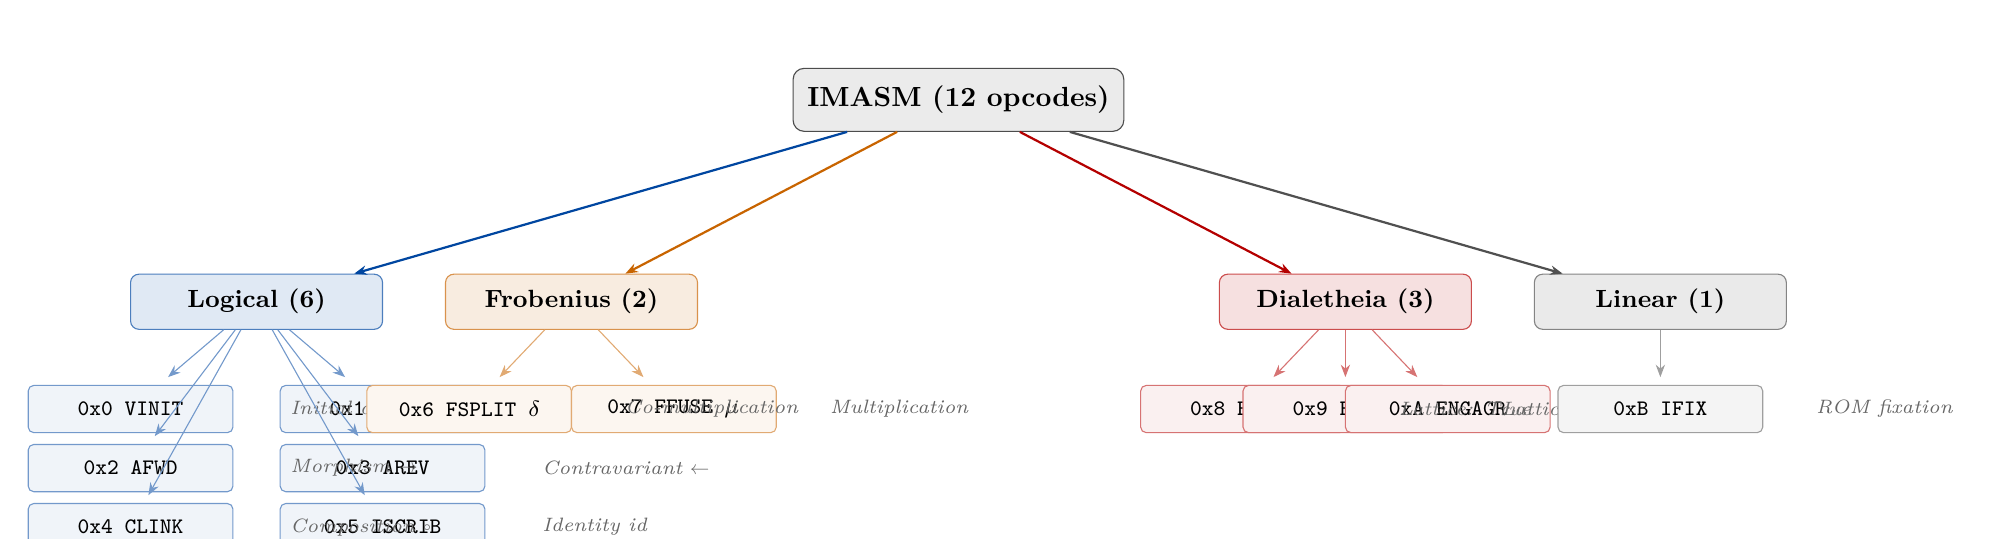
\begin{tikzpicture}[
  root/.style={rectangle, draw=black!70, fill=black!8, rounded corners=4pt,
               font=\bfseries, minimum width=4.2cm, minimum height=0.8cm, align=center},
  fam/.style={rectangle, draw=#1!70, fill=#1!12, rounded corners=3pt,
              font=\bfseries\small, minimum width=3.2cm, minimum height=0.7cm, align=center},
  prim/.style={rectangle, draw=#1!55, fill=#1!6, rounded corners=2pt,
               font=\ttfamily\footnotesize, minimum width=2.6cm, minimum height=0.6cm, align=center, outer sep=3pt},
  ea/.style={-{Stealth[length=4.5pt]}, thick, #1},
  anno/.style={font=\scriptsize\itshape, text=black!60, align=left}
]

\node[root] (root) {IMASM (12 opcodes)};

\node[fam=logcol,  below left=1.8cm and 5.2cm of root] (log)  {Logical (6)};
\node[fam=frobcol, below left=1.8cm and 1.2cm of root] (frob) {Frobenius (2)};
\node[fam=dialcol, below right=1.8cm and 1.2cm of root] (dial) {Dialetheia (3)};
\node[fam=lincol,  below right=1.8cm and 5.2cm of root] (lin)  {Linear (1)};

\draw[ea=logcol]  (root)--(log);
\draw[ea=frobcol] (root)--(frob);
\draw[ea=dialcol] (root)--(dial);
\draw[ea=lincol]  (root)--(lin);

\node[prim=logcol, below=0.6cm of log, xshift=-1.6cm] (n00) {0x0 VINIT};
\node[prim=logcol, below=0.6cm of log, xshift= 1.6cm] (n01) {0x1 TANCH};
\node[prim=logcol, below=1.35cm of log, xshift=-1.6cm] (n02) {0x2 AFWD};
\node[prim=logcol, below=1.35cm of log, xshift= 1.6cm] (n03) {0x3 AREV};
\node[prim=logcol, below=2.1cm of log, xshift=-1.6cm] (n04) {0x4 CLINK};
\node[prim=logcol, below=2.1cm of log, xshift= 1.6cm] (n05) {0x5 ISCRIB};

\node[anno, right=0.5cm of n00] {Initial object $\emptyset$};
\node[anno, right=0.5cm of n01] {Terminal anchor $\top$};
\node[anno, right=0.5cm of n02] {Morphism $\to$};
\node[anno, right=0.5cm of n03] {Contravariant $\leftarrow$};
\node[anno, right=0.5cm of n04] {Composition $\circ$};
\node[anno, right=0.5cm of n05] {Identity \textrm{id}};

\foreach \n in {n00,n01,n02,n03,n04,n05} \draw[ea=logcol!55,thin] (log)--(\n);

\node[prim=frobcol, below=0.6cm of frob, xshift=-1.3cm] (n06) {0x6 FSPLIT $\delta$};
\node[prim=frobcol, below=0.6cm of frob, xshift= 1.3cm] (n07) {0x7 FFUSE $\mu$};
\node[anno, right=0.45cm of n06] {Co-multiplication};
\node[anno, right=0.45cm of n07] {Multiplication};

\node[prim=dialcol, below=0.6cm of dial, xshift=-1.3cm] (n08) {0x8 EVALT};
\node[prim=dialcol, below=0.6cm of dial]                 (n09) {0x9 EVALF};
\node[prim=dialcol, below=0.6cm of dial, xshift= 1.3cm] (n0A) {0xA ENGAGR};
\node[anno, right=0.45cm of n08] {Lattice: True};
\node[anno, right=0.45cm of n09] {Lattice: False};
\node[anno, right=0.45cm of n0A] {Lattice: Both};

\node[prim=lincol, below=0.6cm of lin] (n0B) {0xB IFIX};
\node[anno, right=0.45cm of n0B] {ROM fixation};

\foreach \n in {n06,n07} \draw[ea=frobcol!55,thin] (frob)--(\n);
\foreach \n in {n08,n09,n0A} \draw[ea=dialcol!55,thin] (dial)--(\n);
\draw[ea=lincol!55,thin] (lin)--(n0B);

\end{tikzpicture}
\caption{The twelve IMASM opcodes in four structural families. All nine systems map their token families to these twelve operations.}
\label{fig:taxonomy}
\end{figure}

\subsection{The Tri-Phase Flux Register}

\begin{figure}[htbp]
\centering
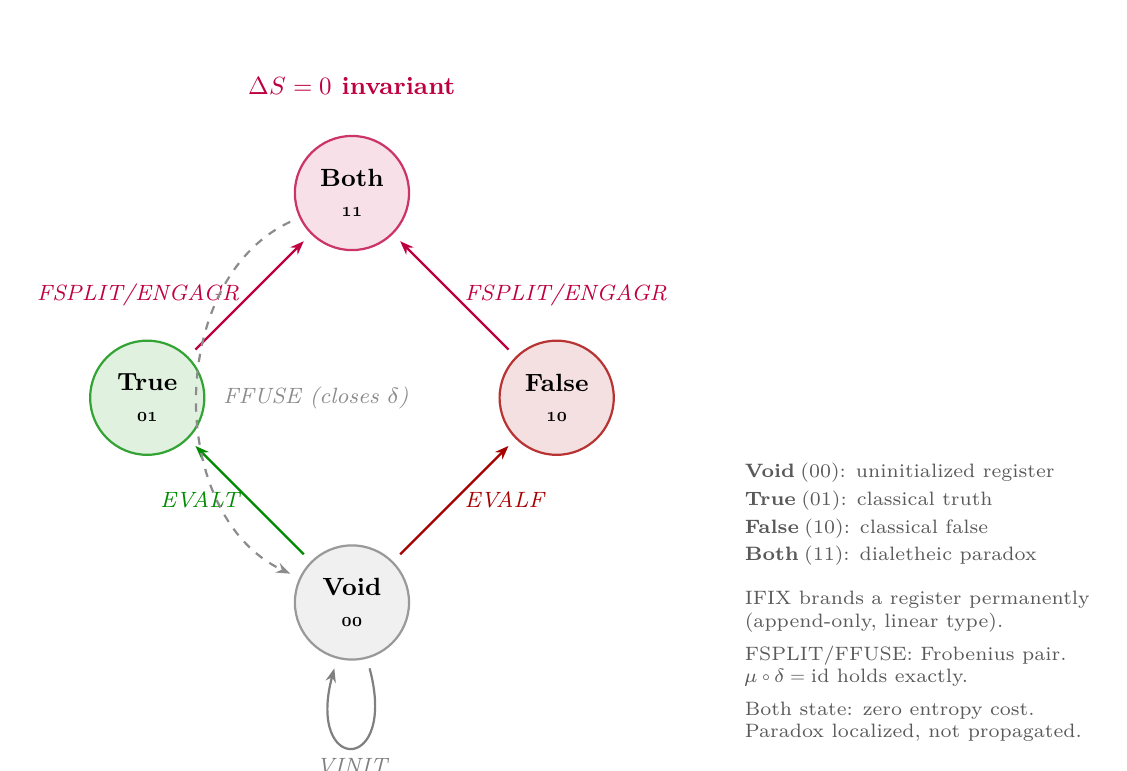
\begin{tikzpicture}[
  st/.style={circle, draw=#1!80, fill=#1!12, thick, minimum size=1.45cm,
             font=\bfseries\small, align=center, outer sep=4pt},
  ar/.style={-{Stealth[length=5pt]}, thick, #1},
  lb/.style={font=\footnotesize\itshape, text=#1}
]
\node[st=gray]           (V) at (0,0)    {Void\\{\tiny 00}};
\node[st=green!55!black] (T) at (-2.6,2.6) {True\\{\tiny 01}};
\node[st=red!65!black]   (F) at ( 2.6,2.6) {False\\{\tiny 10}};
\node[st=purple]         (B) at (0,5.2)    {Both\\{\tiny 11}};

\draw[ar=green!55!black] (V) -- node[lb=green!55!black,left] {EVALT} (T);
\draw[ar=red!65!black]   (V) -- node[lb=red!65!black,right]  {EVALF} (F);
\draw[ar=purple] (T) -- node[lb=purple,left]  {FSPLIT/ENGAGR} (B);
\draw[ar=purple] (F) -- node[lb=purple,right] {FSPLIT/ENGAGR} (B);
\draw[ar=black!45, dashed] (B) edge[bend right=65]
    node[lb=black!45,right=0.2cm] {FFUSE (closes $\delta$)} (V);
\draw[ar=black!50, thick] (V) edge[loop below,looseness=8]
    node[lb=black!50,below] {VINIT} (V);

\node[font=\small\bfseries, above=0.25cm of B, text=purple] {$\Delta S = 0$ invariant};

\node[font=\scriptsize, right=4.0cm of V, align=left, text=black!65] {
\textbf{Void}\;(00): uninitialized register\\[2pt]
\textbf{True}\;(01): classical truth\\[2pt]
\textbf{False}\;(10): classical false\\[2pt]
\textbf{Both}\;(11): dialetheic paradox\\[8pt]
IFIX brands a register permanently\\
(append-only, linear type).\\[4pt]
FSPLIT/FFUSE: Frobenius pair.\\
$\mu \circ \delta = \mathrm{id}$ holds exactly.\\[4pt]
Both state: zero entropy cost.\\
Paradox localized, not propagated.
};
\end{tikzpicture}
\caption{The Tri-Phase Flux Register state lattice. Four states, two bits. The Both state is the grammar's paraconsistent core.}
\label{fig:triphase}
\end{figure}

\subsection{The Frobenius Condition and Bootstrap Sequence}

\begin{figure}[htbp]
\centering
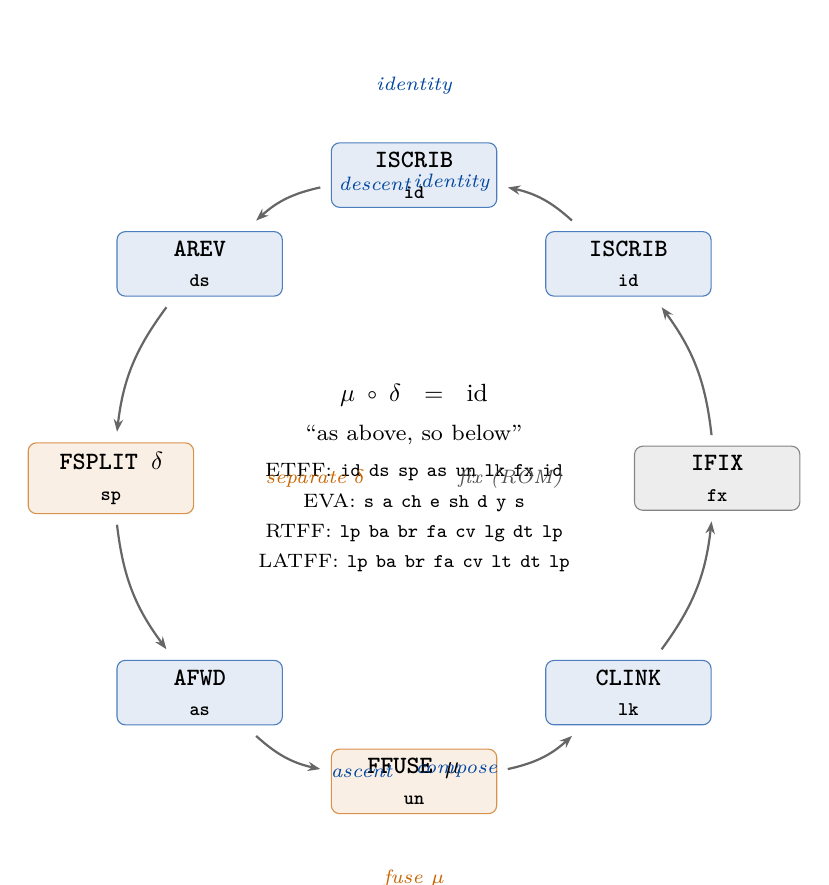
\begin{tikzpicture}[
  nd/.style={rectangle, draw=#1!70, fill=#1!10, rounded corners=3pt,
             font=\ttfamily\small\bfseries, minimum width=2.1cm, minimum height=0.75cm, align=center, outer sep=4pt},
  ar/.style={-{Stealth[length=4.5pt]}, thick, black!60, bend right=15},
  lbl/.style={font=\scriptsize\itshape, text=#1, align=center}
]
\def\r{3.85}

\node[nd=logcol]  (id1)    at ({-\r*sin(  0)},{ \r*cos(  0)}) {ISCRIB\\{\scriptsize id}};
\node[nd=logcol]  (arev)   at ({-\r*sin( 45)},{ \r*cos( 45)}) {AREV\\{\scriptsize ds}};
\node[nd=frobcol] (fsplit) at ({-\r*sin( 90)},{ \r*cos( 90)}) {FSPLIT $\delta$\\{\scriptsize sp}};
\node[nd=logcol]  (afwd)   at ({-\r*sin(135)},{ \r*cos(135)}) {AFWD\\{\scriptsize as}};
\node[nd=frobcol] (ffuse)  at ({-\r*sin(180)},{ \r*cos(180)}) {FFUSE $\mu$\\{\scriptsize un}};
\node[nd=logcol]  (clink)  at ({-\r*sin(225)},{ \r*cos(225)}) {CLINK\\{\scriptsize lk}};
\node[nd=lincol]  (ifix)   at ({-\r*sin(270)},{ \r*cos(270)}) {IFIX\\{\scriptsize fx}};
\node[nd=logcol]  (id2)    at ({-\r*sin(315)},{ \r*cos(315)}) {ISCRIB\\{\scriptsize id}};

\foreach \a/\b in {id1/arev,arev/fsplit,fsplit/afwd,afwd/ffuse,ffuse/clink,clink/ifix,ifix/id2,id2/id1}
  \draw[ar] (\a) to (\b);

\node[align=center, font=\small, text width=4.8cm] at (0,0) {
    $\mu \circ \delta = \mathrm{id}$\\[3pt]
    {\footnotesize ``as above, so below''}\\[2pt]
    {\scriptsize ETFF: \texttt{id ds sp as un lk fx id}}\\
    {\scriptsize EVA: \texttt{s a ch e sh d y s}}\\
    {\scriptsize RTFF: \texttt{lp ba br fa cv lg dt lp}}\\
    {\scriptsize LATFF: \texttt{lp ba br fa cv lt dt lp}}
};

\node[lbl=logcol, above=0.35cm of id1] {identity};
\node[lbl=logcol, above right=0.25cm and 0.45cm of arev] {descent};
\node[lbl=frobcol, right=0.65cm of fsplit] {separate $\delta$};
\node[lbl=logcol, below right=0.25cm and 0.35cm of afwd] {ascent};
\node[lbl=frobcol, below=0.45cm of ffuse] {fuse $\mu$};
\node[lbl=logcol, below left=0.25cm and 0.35cm of clink] {compose};
\node[lbl=lincol, left=0.65cm of ifix] {fix (ROM)};
\node[lbl=logcol, above left=0.25cm and 0.45cm of id2] {identity};

\end{tikzpicture}
\caption{The bootstrap sequence: $\mu \circ \delta = \mathrm{id}$ as eight-step categorical assembly. All four IMASM token systems express the same eight instructions; their surface tokens differ, their operational content does not.}
\label{fig:bootstrap}
\end{figure}

% ─────────────────────────────────────────────────────────────────────────────
\section{The Five Founding Systems}
\label{sec:founding}
% ─────────────────────────────────────────────────────────────────────────────

\begin{figure}[htbp]
\centering
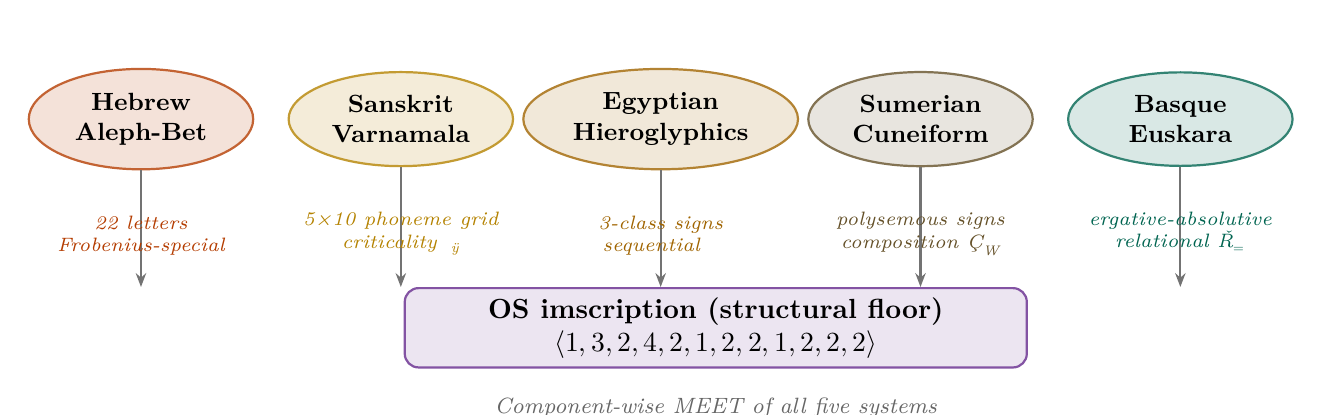
\begin{tikzpicture}[
  sys/.style={ellipse, draw=#1!80, fill=#1!15, thick,
              font=\small\bfseries, minimum width=2.85cm, minimum height=1.05cm, align=center},
  os/.style={rectangle, draw=oscol!80, fill=oscol!12, rounded corners=5pt, thick,
             font=\bfseries, minimum width=7.9cm, minimum height=0.98cm, align=center},
  ar/.style={-{Stealth[length=5pt]}, thick, black!55},
  lb/.style={font=\scriptsize\itshape, text=#1, align=center}
]

\node[sys=hebrewcol]  (heb) at (-7.3, 3.3) {Hebrew\\Aleph-Bet};
\node[sys=sanskritcol](san) at (-4.0, 3.3) {Sanskrit\\Varnamala};
\node[sys=egyptcol]   (egy) at (-0.7, 3.3) {Egyptian\\Hieroglyphics};
\node[sys=cuneicol]   (cun) at ( 2.6, 3.3) {Sumerian\\Cuneiform};
\node[sys=basquecol]  (bas) at ( 5.9, 3.3) {Basque\\Euskara};

\node[os] (os) at (0, 0.65)
    {OS imscription (structural floor)\\
     $\langle 1,3,2,4,2,1,2,2,1,2,2,2 \rangle$};

\foreach \s in {heb,san,egy,cun,bas}
  \draw[ar] (\s.south) -- (os.north-|\s.south);

\node[lb=black!60, below=0.25cm of os]
    {\footnotesize Component-wise MEET of all five systems};

\node[lb=hebrewcol,  below=0.45cm of heb]  {22 letters\\Frobenius-special};
\node[lb=sanskritcol,below=0.45cm of san]  {5×10 phoneme grid\\criticality $\text{⊙}_\text{ÿ}$};
\node[lb=egyptcol,   below=0.45cm of egy]  {3-class signs\\sequential $\text{ɢ}_\text{ˌ}$};
\node[lb=cuneicol,   below=0.45cm of cun]  {polysemous signs\\composition $\text{Ç}_\text{W}$};
\node[lb=basquecol,  below=0.45cm of bas]  {ergative-absolutive\\relational $\text{Ř}_{=}$};

\end{tikzpicture}
\caption{The five founding systems converging to the OS imscription via component-wise MEET. Each system contributes structural constraints; their intersection is the grammar's invariant floor.}
\label{fig:founding}
\end{figure}

\subsection{Hebrew: The Aleph-Bet}

The 22-letter Hebrew Aleph-Bet is the oldest known writing system organized by explicit categorical principle rather than by phonological convention alone. The \emph{Sefer Yetzirah} (Book of Formation), the earliest surviving Kabbalistic text, describes the 22 letters as the ``building blocks of creation'' --- not as an alphabet for representing sound, but as a generative combinatorial system from which all structure is derived.

The Sefer Yetzirah partitions the 22 letters into three structural tiers: 3 \emph{Mothers} (Aleph, Mem, Shin), 7 \emph{Doubles} (Beth, Gimel, Dalet, Kaph, Pe, Resh, Tav), and 12 \emph{Elementals}. The grammar reads this partition structurally:

\begin{itemize}
\item \textbf{3 Mothers}: Aleph (air, $\emptyset$) $\to$ VINIT; Mem (water, $\leftarrow$) $\to$ AREV; Shin (fire, $\to$) $\to$ AFWD. The three archaic elements are the three morphism types: initial, forward, and reverse.
\item \textbf{7 Doubles} (letters with two phonetic values, hard/soft): the dual-valued letter is a register in the Both state --- dual-rail co-multiplication. Seven FSPLIT/FFUSE pairs.
\item \textbf{12 Elementals}: the twelve grammatical-categorical primitives directly. The assignment is structural, not phonetic: each Elemental letter corresponds to a direction in the 12-dimensional primitive space.
\end{itemize}

The JOIN of all 22 Hebrew letters (the maximal imscription the alphabet can support) imscribes with $\text{Φ}_\}$ (Frobenius-special, both gates open) and $\text{Ω}_z$ (integer winding, closed cycle from Aleph to Tav and back). The MEET contribution to the OS floor: $\text{Þ}_¨$ (bounded domain), $\text{Φ}_\}$ (Frobenius-special), $\text{⊙}_\text{ÿ}$ (self-modeling criticality --- the alphabet that describes all creation must describe itself).

\subsection{Sanskrit: The Varnamala}

The Sanskrit Varnamala (``garland of phonemes'') is a 50-phoneme system organized in a $5 \times 10$ matrix by place and manner of articulation. This is not merely convenient linguistic classification --- it is a categorical lattice. The rows (guttural, palatal, retroflex, dental, labial) and columns (stop/aspirated/voiced/nasal + semivowels/fricatives/laryngeals) form a product structure: each phoneme is a morphism from a place of articulation to a manner of realization.

The Sanskrit varnamala's structural character:
\begin{itemize}
\item The $5 \times 10$ grid is a Cartesian product of two categorical axes: $\text{Ř}$ (relational mode, bidirectional morphism) at full symmetric closure.
\item The nasal phonemes at each row are the identity morphisms: they resonate but do not transform. These are ISCRIB.
\item Stops (hard closure) are IFIX: the articulator fully stops airflow, fixing the vocal tract in a particular position.
\item The aspirated cognates (kh, gh, ch, etc.) are FSPLIT from the stops: same place, split manner. Each pair is a Frobenius $\delta$/$\mu$ couple.
\item The semivowel and fricative columns are AFWD/AREV: directional flow without full closure.
\end{itemize}

The Sanskrit varnamala imscribes with $\text{Γ}_\text{ʔ}$ (universal scope: the phoneme grid aspires to completeness across all possible articulations) and $\text{⊙}_\text{ÿ}$ (criticality: the phonological system is exactly at the self-organizing threshold where phonemic distinctions become stable). Its MEET contribution: systematic $\text{Γ}_\text{ʔ}$ scope and $\text{ɢ}_\text{ˌ}$ (sequential interaction).

\subsection{Egyptian: The Tripartite System}

Egyptian hieroglyphics operate on a three-class architecture: \emph{phonograms} (signs for sound), \emph{logograms} (signs for meaning), and \emph{determinatives} (silent classifier signs that fix semantic register). The grammar reads this three-class structure directly:

\begin{itemize}
\item \textbf{Phonograms}: unilateral (single consonant), bilateral (two consonants), and trilateral (three consonants). These are morphism chains: AFWD for unilateral, CLINK for bilateral (composition of two), FSPLIT for trilateral (fork to three paths).
\item \textbf{Logograms}: signs used for their direct meaning. These are ISCRIB (identity): the sign is what it depicts, without transformation.
\item \textbf{Determinatives}: silent signs placed at the end of words to classify semantic register. A word about a city gets the city-wall determinative; a word about a person gets the seated-man determinative. This is IFIX: the determinative \emph{fixes} the semantic type, appending a permanent classification to the word. Determinatives cannot be removed without changing meaning.
\end{itemize}

The trilateral root system (most Egyptian words built from three consonants) has direct Frobenius structure: the three-consonant root is a $\delta$-split from the archaic biliteral, and word formation by insertion of vowels and affixes is $\mu$-fusion back to a single surface form. $\mu \circ \delta = \mathrm{id}$: the trilateral root and its derivations return to the original meaning under the Frobenius law.

Egyptian's MEET contribution: $\text{ɢ}_\text{ˌ}$ (sequential composition, since Egyptian word-order is rigidly head-initial morpheme-sequential) and $\text{Σ}_\text{ï}$ (many-to-many stoichiometry: one root, many forms; one sound, many meanings).

\subsection{Sumerian Cuneiform: The Polysemous Sign}

Sumerian cuneiform is the oldest known writing system, emerging around 3400~BCE in lower Mesopotamia. Its structural contribution to the grammar lies in its \emph{polysemy}: a single cuneiform sign can carry logographic, syllabic, and determinative readings simultaneously. The sign for ``mouth'' (KA) also reads ``word,'' ``tooth,'' ``voice,'' and the syllable \emph{ka}. This is not ambiguity --- it is \emph{superposition}, the same register holding multiple valid states.

The grammar reads this as the Both state: the polysemous sign is a register in the $11$ flux state, holding contradictory but simultaneously valid readings without resolving. ENGAGR (paradox engagement) is the primary opcode of cuneiform's logographic core. Disambiguation happens contextually --- which is CLINK (composition with surrounding context) that selects a reading. The determinative sign (an unpronounced classifier, exactly as in Egyptian) is IFIX.

The cuneiform tablet format is itself architecturally significant: text written in rectangular columns, right to left, then the tablet rotated for the next line. This wrapping topology is $\text{Þ}_K$ (nested containment): a bounded domain that wraps to its own interior boundary.

Cuneiform's MEET contribution: $\text{Ç}_\text{W}$ (moderate kinetics, living vibration --- cuneiform was the world's first administrative writing system, actively used for over 3,000 years without significant structural change) and shared $\text{Σ}_\text{ï}$ (many-to-many: one sign, many readings).

\subsection{Basque: The Ergative Isolate}

Basque (Euskara) is the most structurally anomalous language in this analysis. It is a linguistic isolate: no demonstrated genetic relationship to any other living or extinct language. Its ergative-absolutive alignment, agglutinative morphology, and free word order have no clear parallel in any European language family. And yet it imscribes in the grammar.

The key structural feature is the ergative-absolutive case system. In Basque, the \emph{absolutive} marks the subject of intransitive verbs and the object of transitive verbs; the \emph{ergative} marks only the subject of transitive verbs. This is not merely a grammatical quirk --- it is a categorical statement about morphism direction:

\begin{itemize}
\item \textbf{Absolutive}: the ground state. A noun in absolutive is VINIT (initial object, no morphism applied yet).
\item \textbf{Ergative}: the transitive agent. Marks the source of a morphism --- AFWD. The ergative case literally encodes ``this argument is the origin of a forward morphism.''
\item \textbf{Dative, genitive, etc.}: compositional cases built by agglutination from the absolutive. These are CLINK chains: each suffix is a composed morphism.
\end{itemize}

The Basque verb system also encodes the absolutive/ergative distinction on the verb itself (polypersonal agreement), making the full morphism diagram explicit in the surface form: subject, object, indirect object, and their case-relationships are all visible in the conjugated verb. This is $\text{Ř}_{=}$ (bidirectional adjoint pair): the verb simultaneously expresses the forward morphism (ergative → dative) and its adjoint (absolutive reference).

Basque's MEET contribution: $\text{Ř}_{=}$ (full relational adjoint closure) and $\text{Φ}_\}$ (Frobenius-special parity --- the ergative/absolutive split is exactly the categorical split that makes the Frobenius condition syntactically visible).

\subsection{The OS Imscription: Their MEET}

\begin{admonitionbox}[OS Imscription]{oscol}
$\mathrm{MEET}(\text{Hebrew}, \text{Sanskrit}, \text{Egyptian}, \text{Cuneiform}, \text{Basque})$
$= \langle\,1,3,2,4,2,1,2,2,1,2,2,2\,\rangle$
\end{admonitionbox}

Reading the OS imscription dimension by dimension:

\begin{center}
\small
\begin{tabular}{ll p{7cm}}
\toprule
Primitive & Value & Structural meaning \\
\midrule
\ig{Ð} & 1 ($\text{Ð}_C$) & Triangular (3-dimensional) categorical structure. All five systems are at least 3-category systems. \\
\ig{Þ} & 3 ($\text{Þ}_{\text{¨}}$) & Bounded domain topology. Each system operates within a closed, bounded imscriptive field. \\
\ig{Ř} & 2 ($\text{Ř}_{\text{Ť}}$) & Dagger-category relational mode. All five systems have at least one-sided adjoint pairs. \\
\ig{Φ} & 4 ($\text{Φ}_\}$) & Frobenius-special parity. All five systems instantiate $\mu \circ \delta = \mathrm{id}$ structurally. \\
\ig{ƒ} & 2 ($\text{ƒ}^\text{ż}$) & Quantum-coherent fidelity. The symbol surface maintains phase coherence. \\
\ig{Ç} & 1 ($\text{Ç}_\text{W}$) & Moderate kinetics (living vibration). Not frozen, not explosive. \\
\ig{Γ} & 2 ($\text{Γ}_\text{ʔ}$) & Universal scope. All five systems aspire to totality. \\
\ig{ɢ} & 2 ($\text{ɢ}_\text{ˌ}$) & Sequential interaction. Linear morphism composition. \\
\ig{⊙} & 1 ($\text{⊙}_\text{ÿ}$) & Self-modeling criticality. Each system can describe its own structure. \\
\ig{Ħ} & 2 ($\text{Ħ}_A$) & Two-step chirality. A two-generation temporal embedding (as above $\to$ below $\to$ above). \\
\ig{Σ} & 2 ($\text{Σ}_\text{ï}$) & Many-to-many stoichiometry. Complex morphism ratios. \\
\ig{Ω} & 2 ($\text{Ω}_z$) & Integer winding. Complete cycles, non-trivial topology. \\
\bottomrule
\end{tabular}
\end{center}

% ─────────────────────────────────────────────────────────────────────────────
\section{The Four Engine Corpora}
\label{sec:engines}
% ─────────────────────────────────────────────────────────────────────────────

The four engine corpora each compile independently to the same twelve-opcode IMASM
instruction set. Their register flow graphs are shown below; all use the full compiled
corpus (not a single folio/page/tablet). Nodes are colored by opcode family: blue
(Frobenius), orange (Morphism), green (Identity/Linear), red (Dialetheia), gray
(Bootstrap). Orange FSPLIT edges indicate Frobenius co-multiplication forks.

\begin{table}[htbp]
\centering
\small
\begin{tabular}{llrrrll}
\toprule
System & Token format & Units & Instructions & Component & $d(\cdot,\text{OS})$ & $C$ \\
\midrule
Voynich      & EVA (ch sh o p e a d s t k r y)       & 227 folios   & 44{,}445 & 546n · 694e & 4.31 & $<$1 \\
Rohonc       & RTFF (cr hk fa ba lg lp br cv vt hz cl dt) & 33 pages  &  1{,}650 &  50n ·  50e & 2.09 & $<$1 \\
Linear A     & LATFF (cu hk fa ba lt lp br cv vt hz cl dt) & 53 tablets & 2{,}650 &  50n ·  50e & 0.00 & $<$1 \\
Emerald T.   & ETFF (tr an as ds lk id sp un af ng px fx) & 15 versicles &  460 &  40n ·  41e & 2.44 & 1.0 \\
\bottomrule
\end{tabular}
\caption{Compiled corpus statistics for the four engine systems. Component = nodes · edges
in the largest weakly connected component of the full-corpus register flow graph.}
\label{tab:engines}
\end{table}

\subsection{The Voynich Manuscript (IVTFF → IMASM)}

The Voynich Manuscript (15th~c., \emph{c.}~1404--1438) is compiled via the IVTFF
transcription format (Takahashi \texttt{;H>} lines). EVA characters scan to twelve
opcodes: \texttt{ch}~$\to$~FSPLIT, \texttt{sh}~$\to$~FFUSE, and ten single-character
tokens covering the remaining ten families. The manuscript is the most distant from
the OS floor ($d = 4.31$): its $\text{Þ}_K$ (nested containment topology) and
$\text{Ç}_\text{trap}$ (MBL kinetics) drive it farthest from the structural core.
Despite this distance, its MEET with the OS imscription returns the OS imscription
exactly --- it does not alter the floor.

\begin{figure}[htbp]
\centering
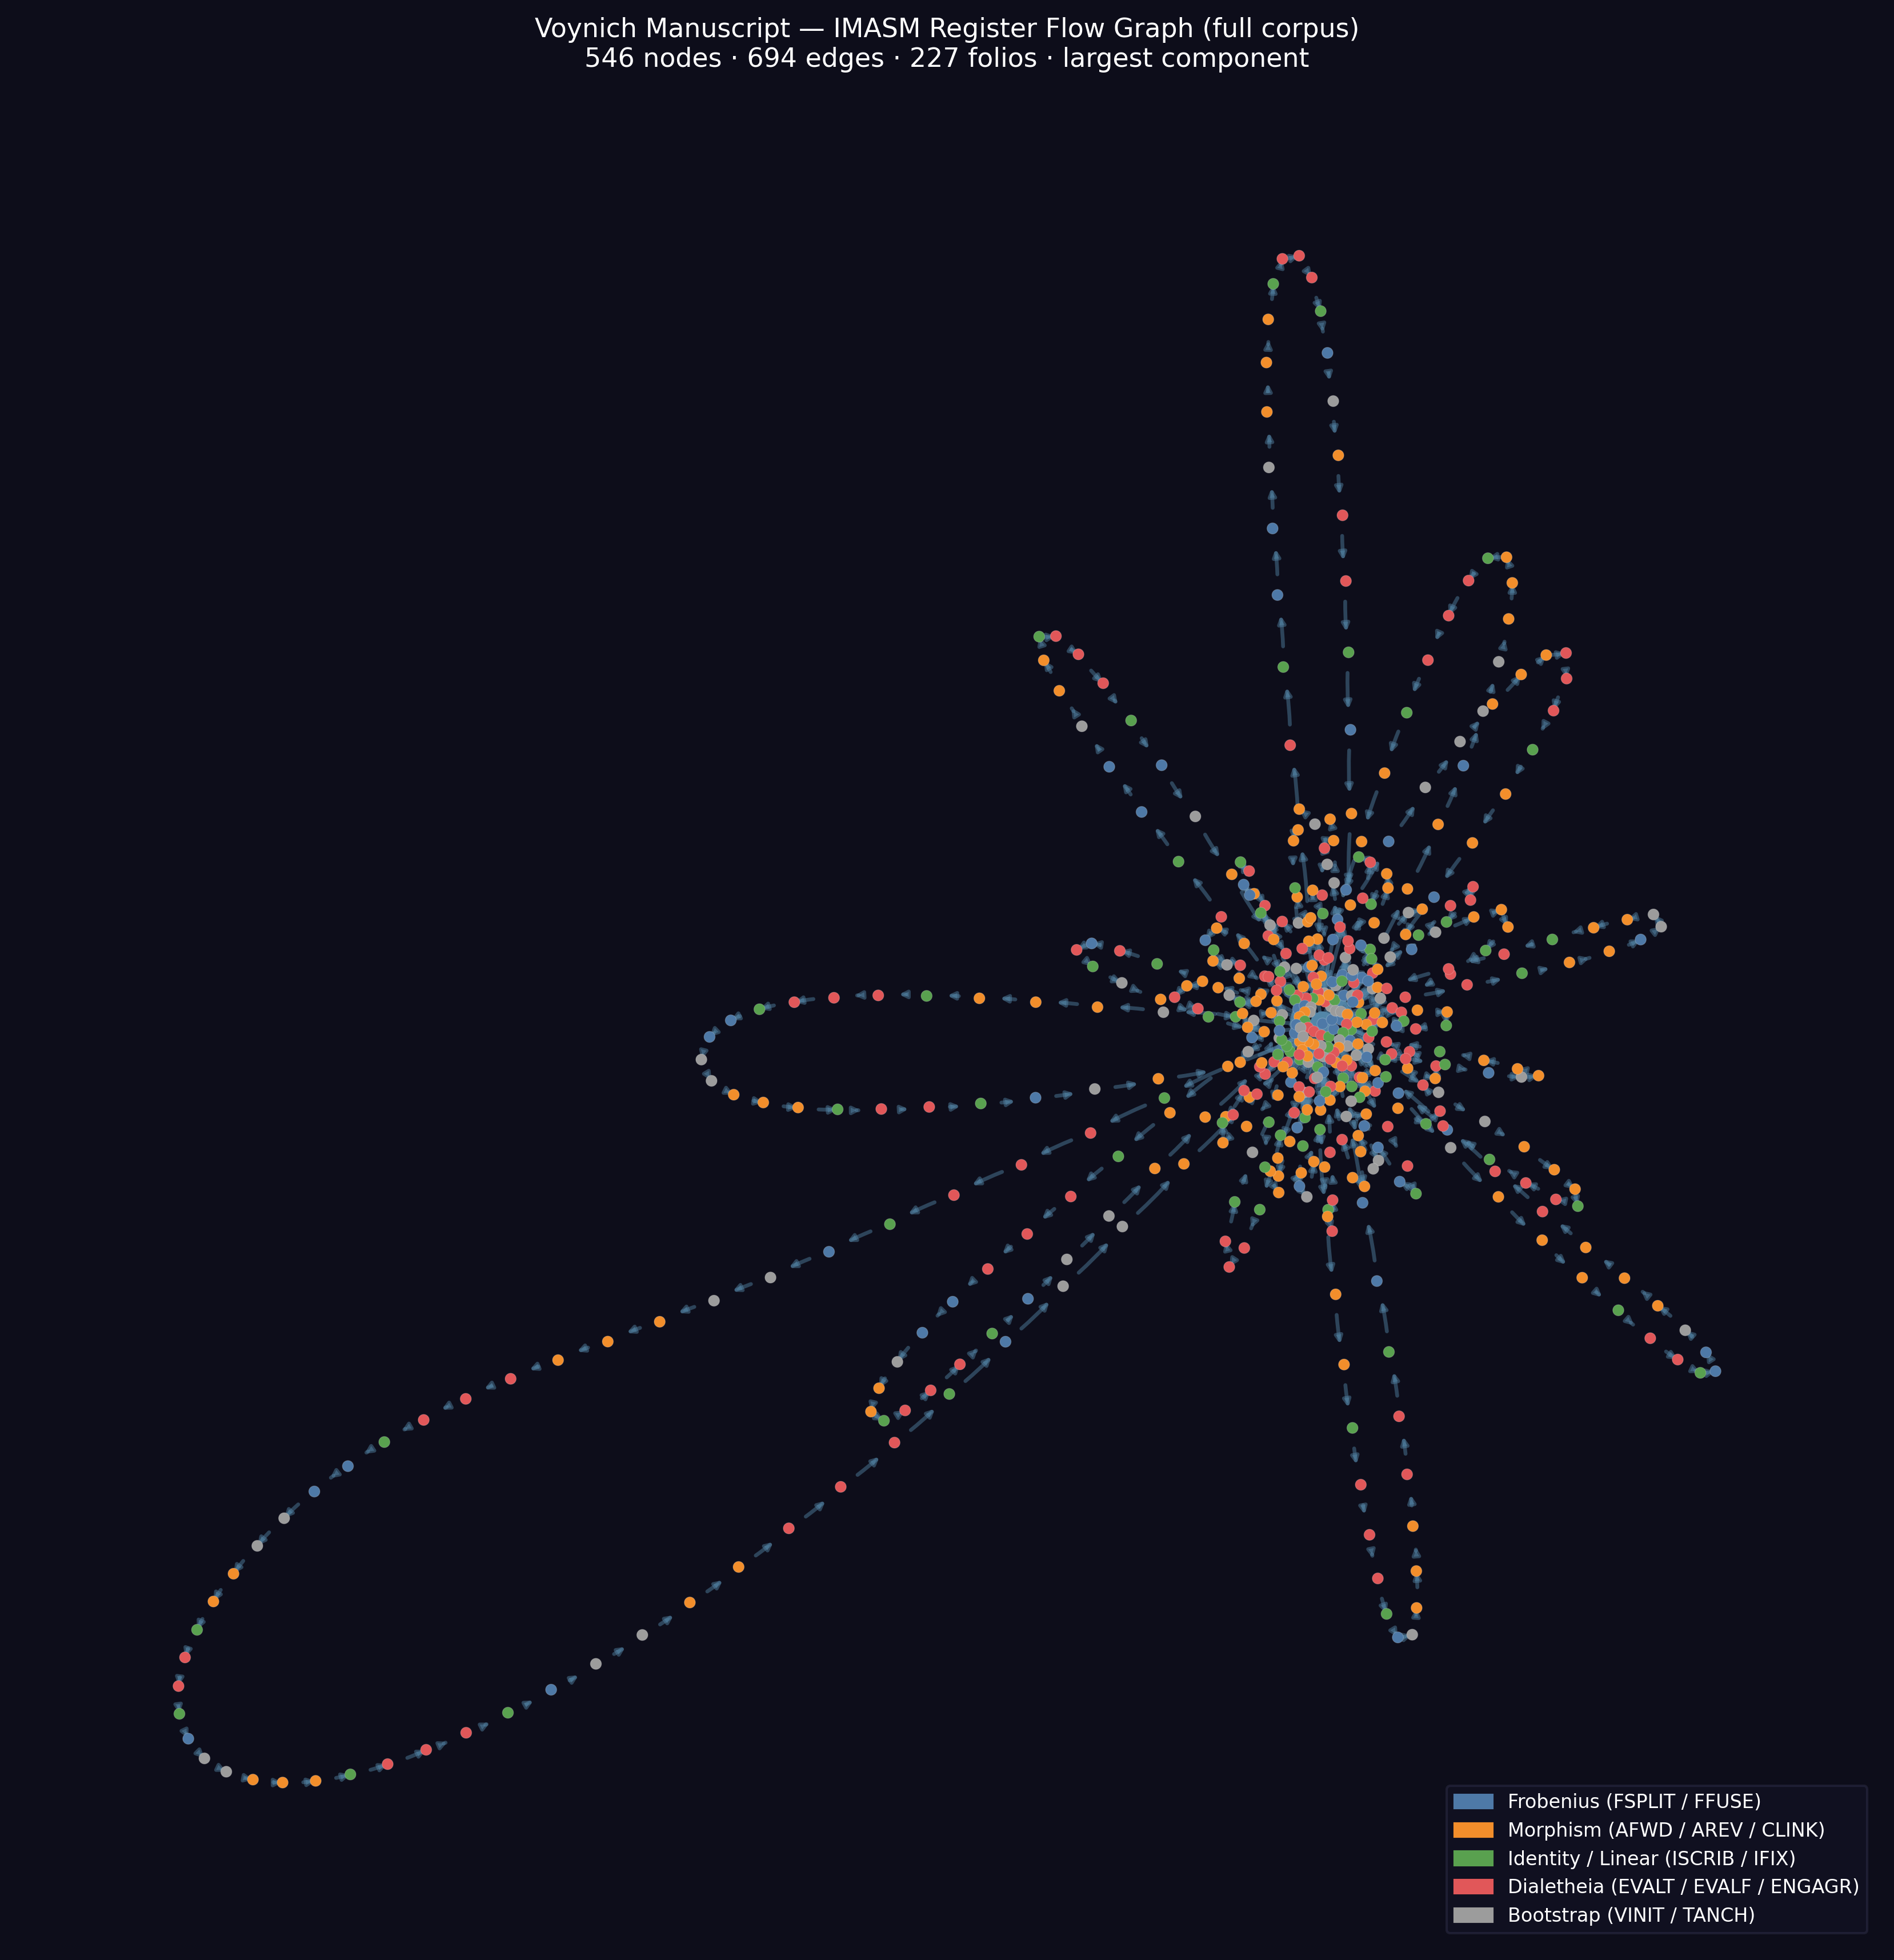
\includegraphics[width=\textwidth,keepaspectratio]{voynich_callgraph_document.png}
\caption{Voynich Manuscript --- IMASM register flow graph, full corpus (227 folios,
44{,}445 instructions). Largest component: 546 nodes, 694 edges. The dense orange
FSPLIT cluster reflects the manuscript's heavy Frobenius co-multiplication signature.}
\label{fig:cfg_voynich}
\end{figure}

\subsection{The Rohonc Codex (RTFF → IMASM)}

The Rohonc Codex (16th--17th~c.) is compiled via RTFF (Rohonc Transcription Folio
Format): 33 pages of symbol sequences. The twelve RTFF visual families (cross/crucifix,
hook/fishhook, forward-arc, backward-arc, ligature, loop/mirror, branch/fork,
convergent, vertical-stroke, horizontal-stroke, closed-loop, dot/point) map directly
to the twelve opcodes. At $d = 2.09$ from the OS floor, the Rohonc Codex is the
closest of the three undeciphered manuscripts to the structural core.

\begin{figure}[htbp]
\centering
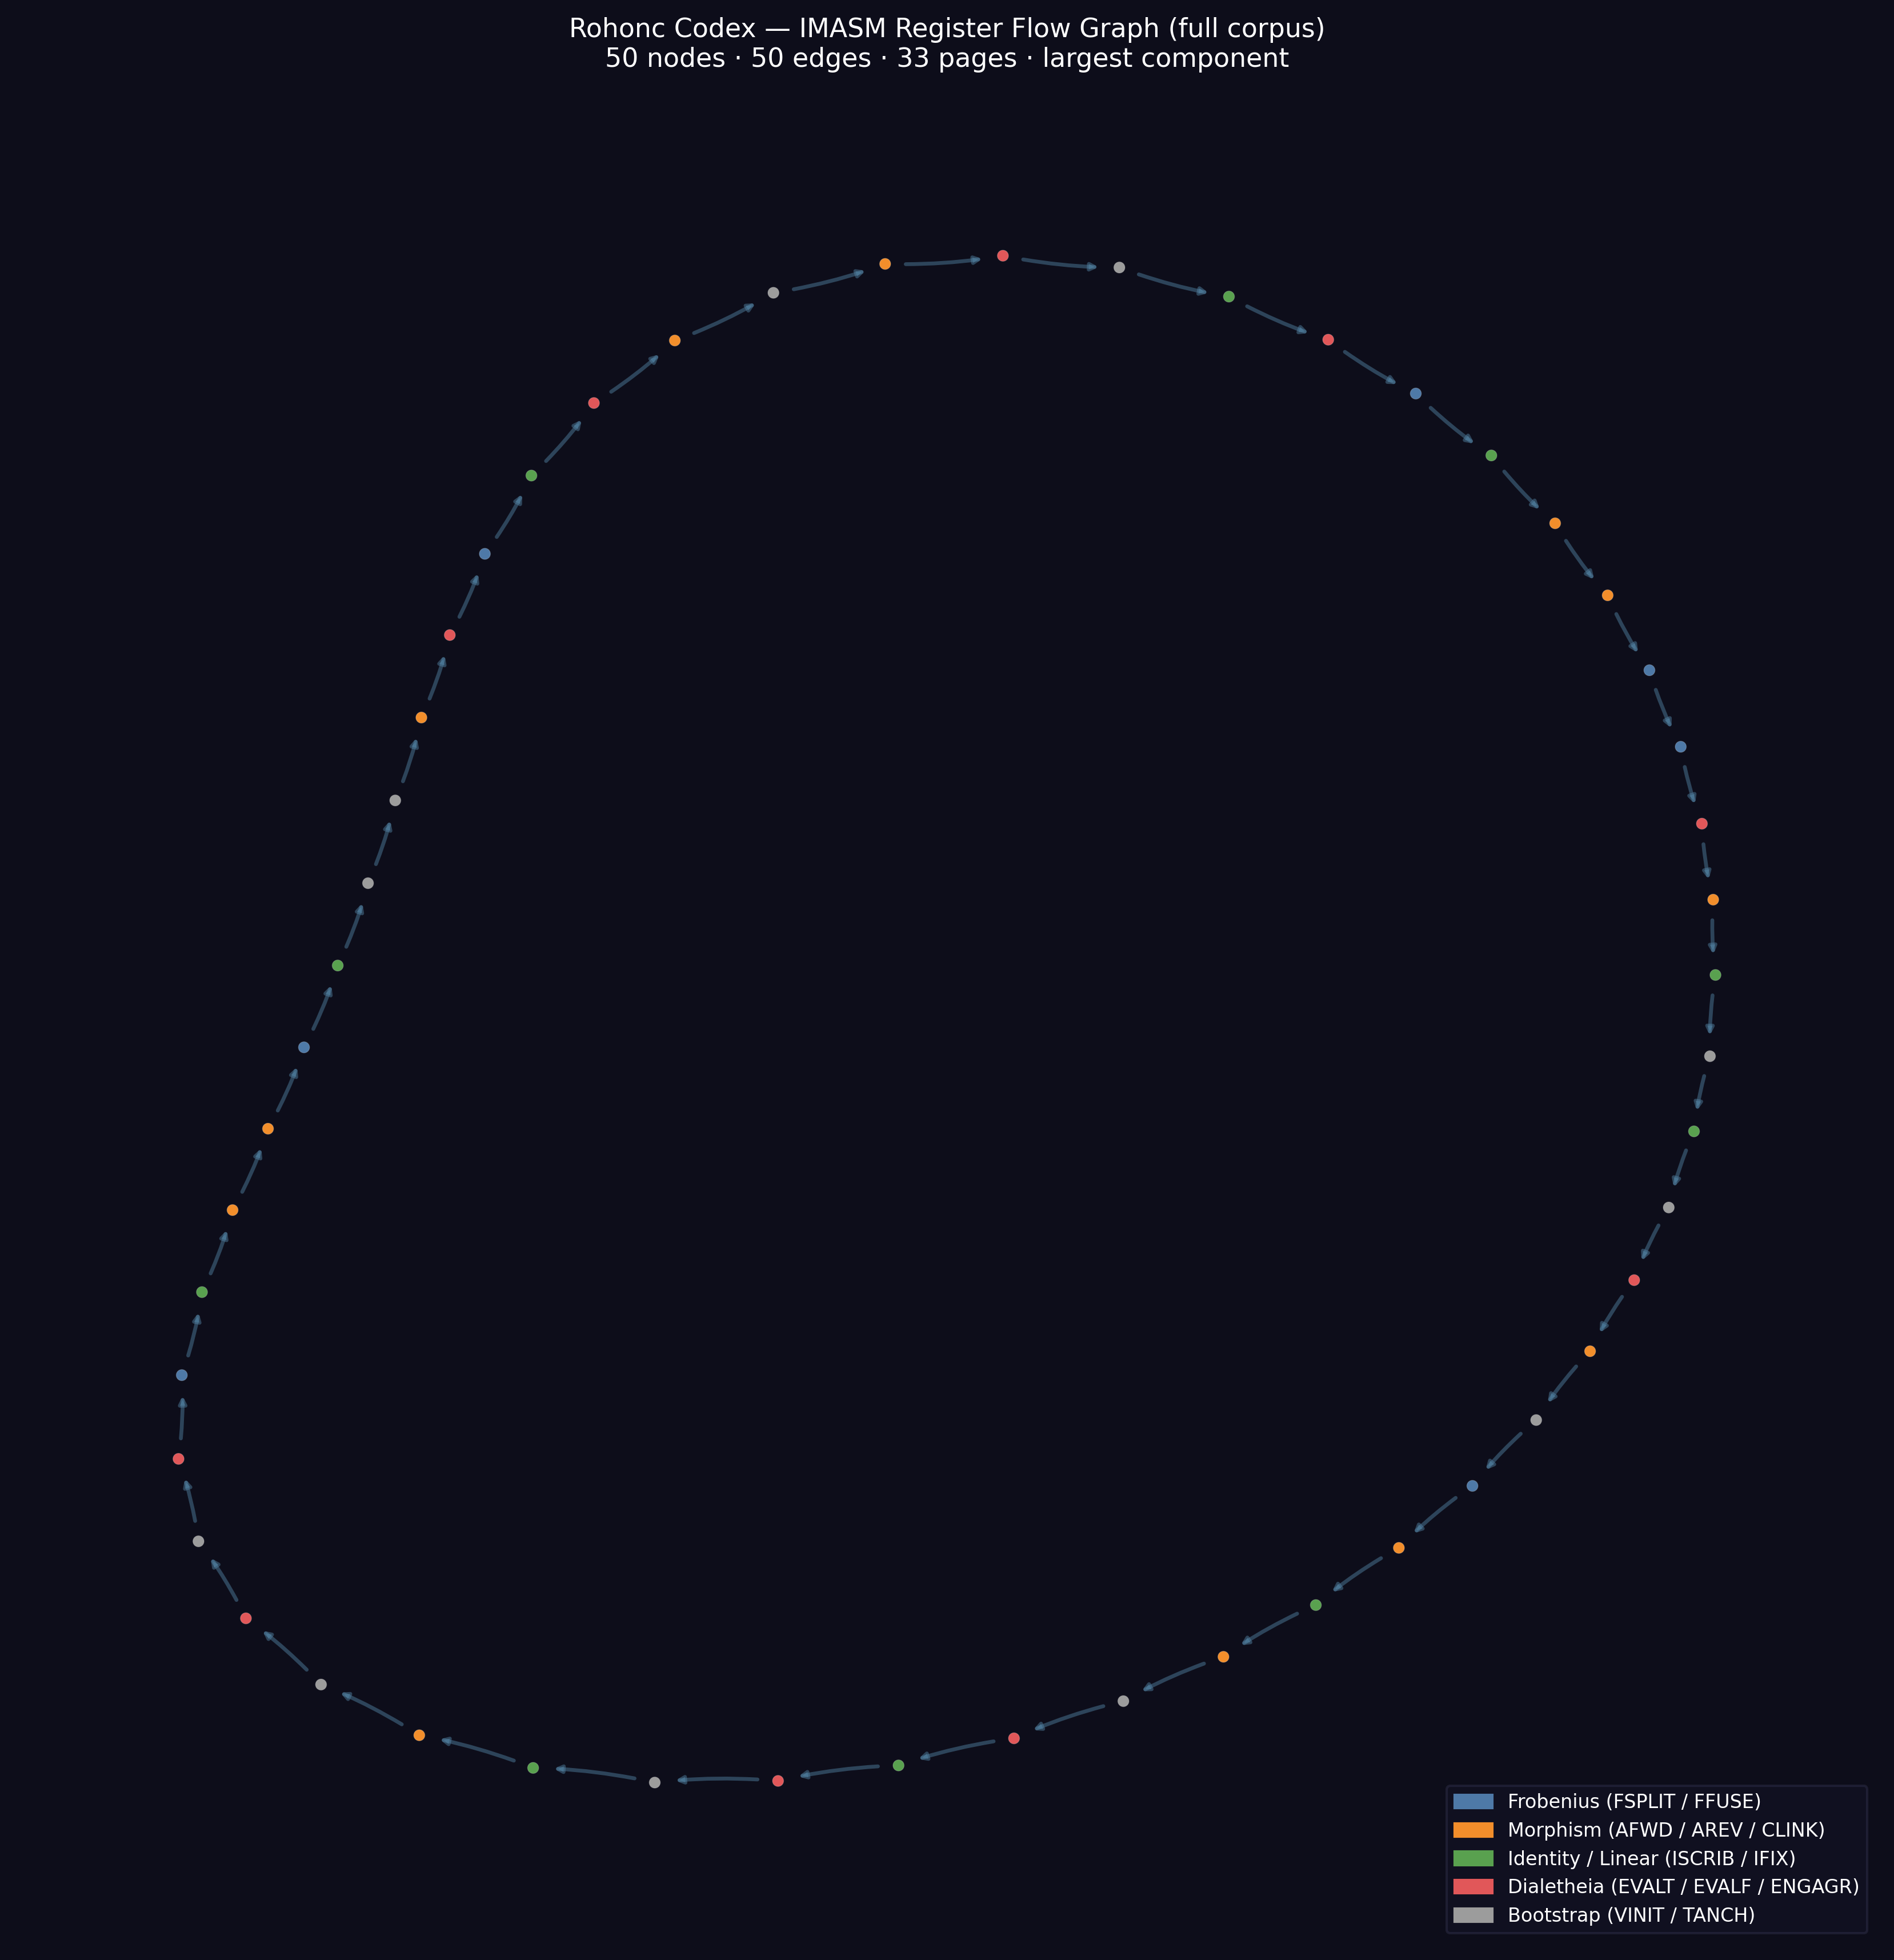
\includegraphics[width=\textwidth,keepaspectratio]{rohonc_callgraph_document.png}
\caption{Rohonc Codex --- IMASM register flow graph, full corpus (33 pages,
1{,}650 instructions). Largest component: 50 nodes, 50 edges. The compact, cyclic
topology reflects the codex's tight bootstrap structure.}
\label{fig:cfg_rohonc}
\end{figure}

\subsection{Linear A (LATFF → IMASM)}

Linear A (Minoan Crete, \emph{c.}~2000--1450~BCE) is compiled via LATFF (Linear A
Tablet Folio Format): 53 tablets. The twelve LATFF sign families (cup/vessel,
hook/arm, forward-arc, backward-arc, lattice/compound, loop/knot, branching,
convergent/triangular, vertical-stroke, horizontal-stroke, closed/circle,
dot/fraction) are the twelve opcodes. Linear A imscribes at $d = 0.00$: it is not
merely close to the OS floor --- it \emph{is} the floor. The Minoan script is the
structural core that the five founding systems converge upon, independently of any
contact or inheritance.

\begin{figure}[htbp]
\centering
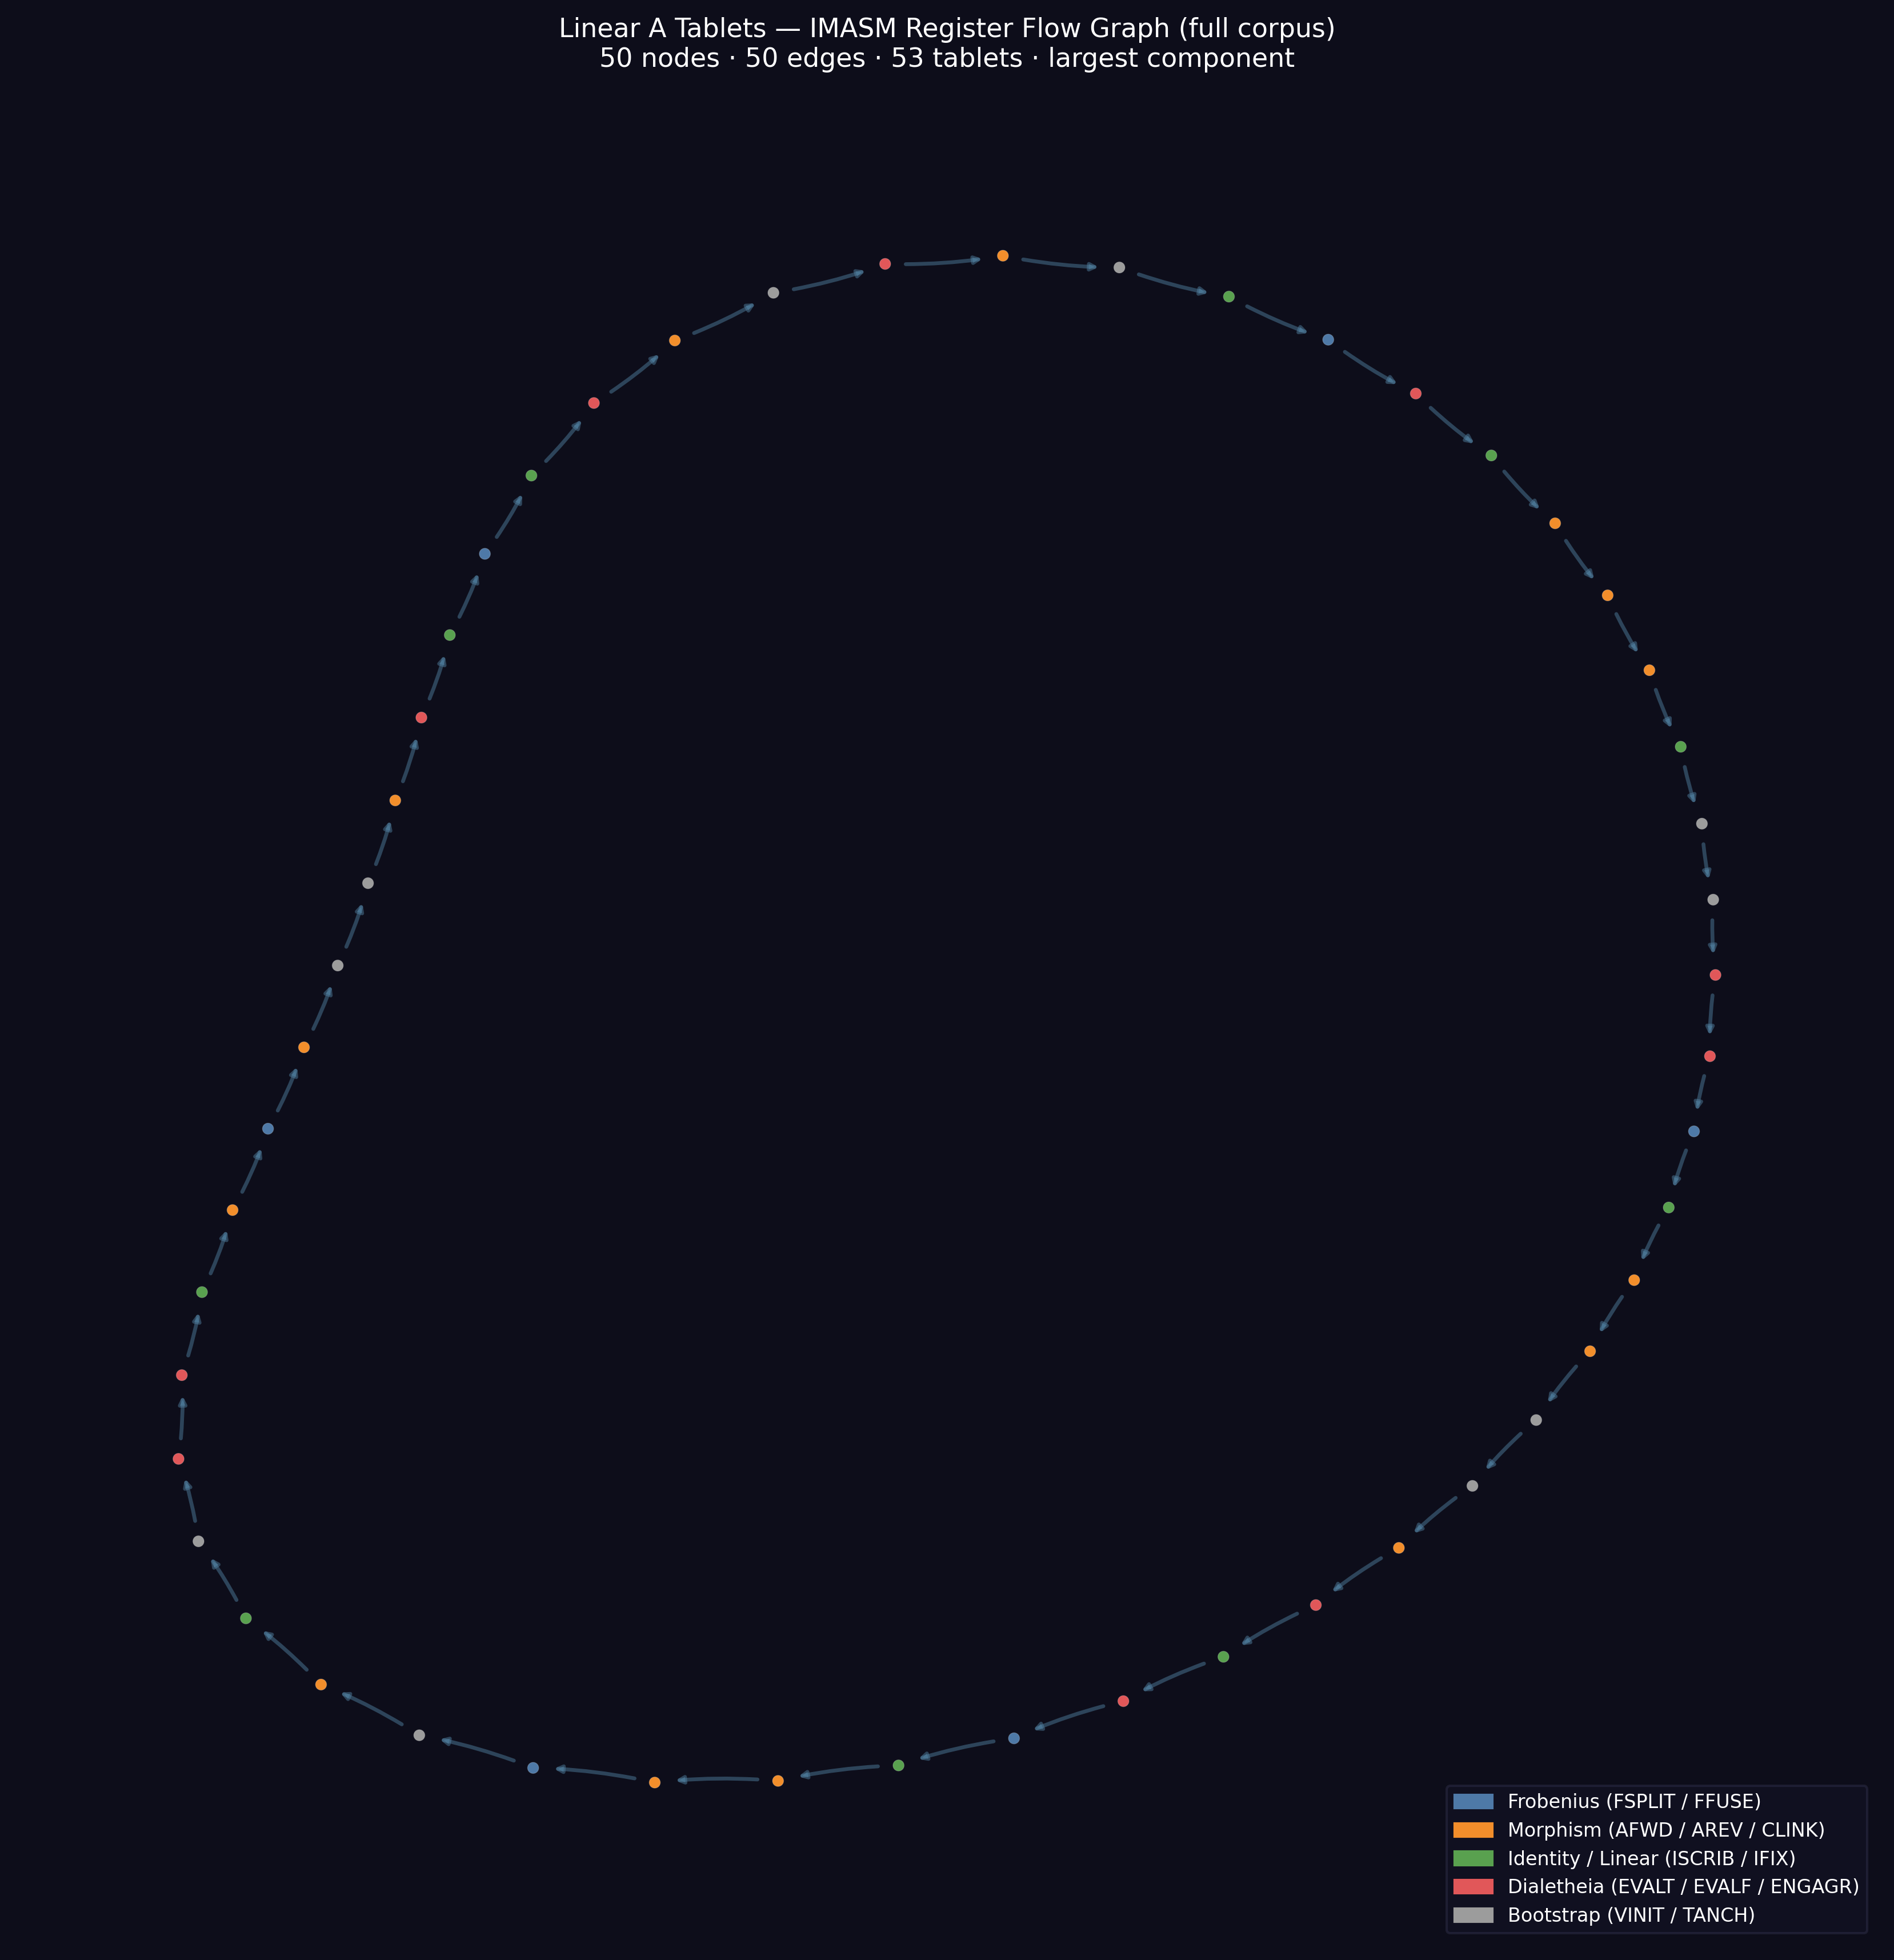
\includegraphics[width=\textwidth,keepaspectratio]{linear_a_callgraph_document.png}
\caption{Linear A --- IMASM register flow graph, full corpus (53 tablets,
2{,}650 instructions). Largest component: 50 nodes, 50 edges. Structurally
identical to the OS floor ($d = 0.00$): the graph topology reflects the same
categorical skeleton as the five founding systems' MEET.}
\label{fig:cfg_lineara}
\end{figure}

\subsection{The Emerald Tablet (ETFF → IMASM)}

The Emerald Tablet (attributed to Jabir ibn Hayyan, \emph{c.}~8th~c.~CE) is compiled
via ETFF (Emerald Tablet Folio Format): 15 versicles. The twelve ETFF rhetorical
families (truth-seal, anchor, ascent, descent, linkage, identity, separation, union,
affirmation, negation, paradox, fixing) map the tablet's cosmological claims to
opcodes. It is the only compiled manuscript with $C = 1.0$ (quantum-coherent fidelity)
and both type gates open. Its central claim --- ``as above, so below'' --- is the
Frobenius condition $\mu \circ \delta = \mathrm{id}$, stated as cosmological law. The
ETFF bootstrap sequence is \texttt{id\,ds\,sp\,as\,un\,lk\,fx\,id}; every other
surface transliteration of the bootstrap resolves to the same eight instructions.

\begin{figure}[htbp]
\centering
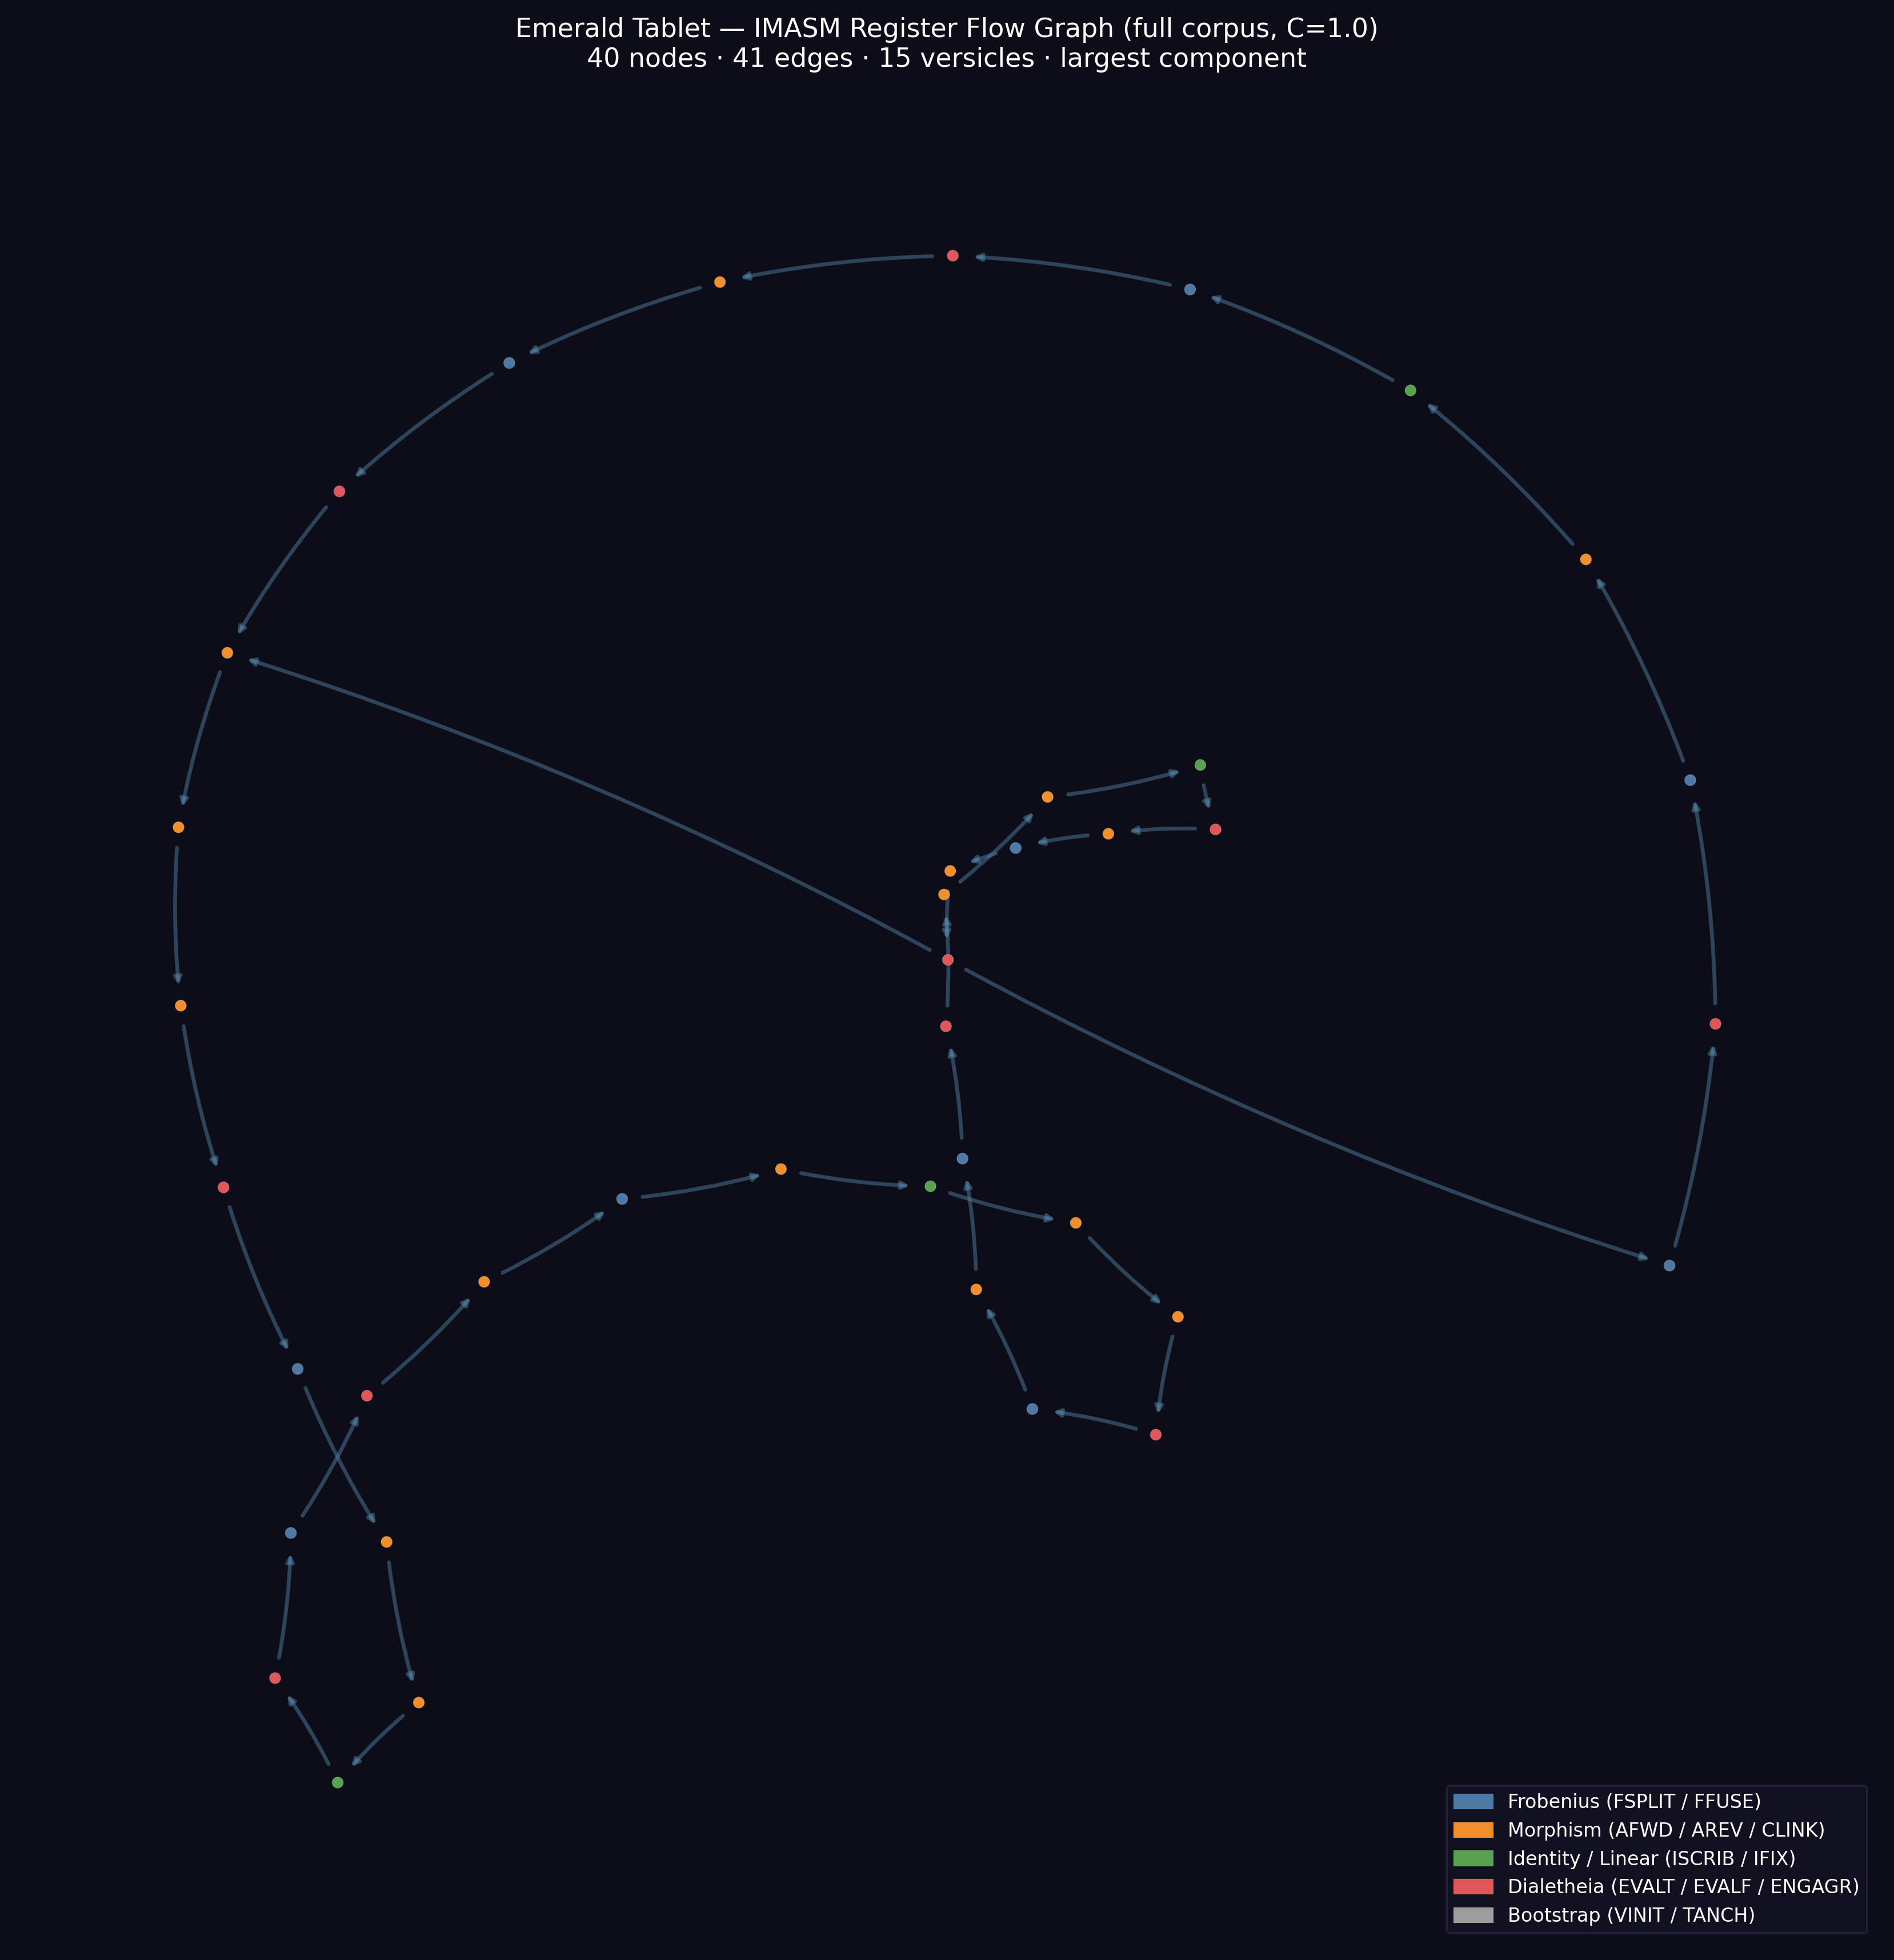
\includegraphics[width=\textwidth,keepaspectratio]{emerald_tablet_callgraph_document.png}
\caption{Emerald Tablet --- IMASM register flow graph, full corpus (15 versicles,
460 instructions). Largest component: 40 nodes, 41 edges. The near-unicyclic
structure reflects $C = 1.0$: both Frobenius gates are open and the graph closes
cleanly --- $\mu \circ \delta = \mathrm{id}$ holds with no broken splits.}
\label{fig:cfg_emerald}
\end{figure}

% MEET Lattice
\begin{figure}[htbp]
\centering
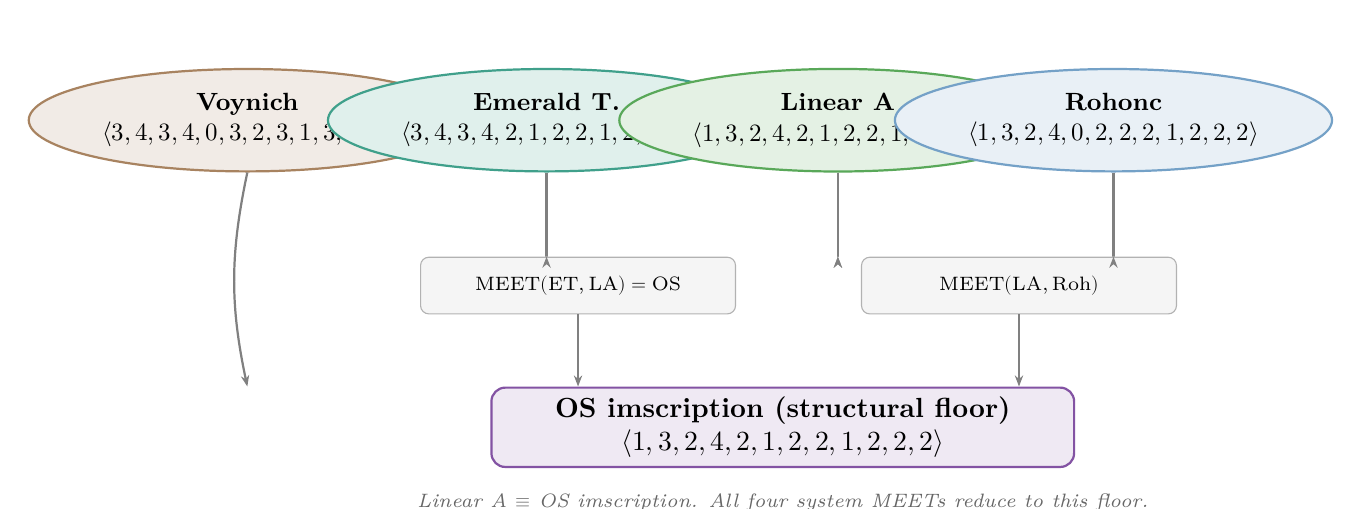
\begin{tikzpicture}[
  sys/.style={ellipse, draw=#1!75, fill=#1!12, thick,
              font=\small\bfseries, minimum width=2.6cm, minimum height=0.95cm, align=center},
  meet/.style={rectangle, draw=gray!60, fill=gray!8, rounded corners=3pt,
               font=\scriptsize, minimum width=4.0cm, minimum height=0.72cm, align=center},
  os/.style={rectangle, draw=oscol!80, fill=oscol!10, rounded corners=5pt, thick,
             font=\bfseries, minimum width=7.4cm, minimum height=0.85cm, align=center},
  ar/.style={-{Stealth[length=4pt]}, thick, black!50},
]

\node[sys=voynich] (voy) at (-5.2, 4.2) {Voynich\\$\langle 3,4,3,4,0,3,2,3,1,3,0,2\rangle$};
\node[sys=emerald] (et)  at (-1.4, 4.2) {Emerald T.\\$\langle 3,4,3,4,2,1,2,2,1,2,2,2\rangle$};
\node[sys=lineara] (la)  at ( 2.3, 4.2) {Linear A\\$\langle 1,3,2,4,2,1,2,2,1,2,2,2\rangle$};
\node[sys=rohonc]  (roh) at ( 5.8, 4.2) {Rohonc\\$\langle 1,3,2,4,0,2,2,2,1,2,2,2\rangle$};

\node[meet] (m1) at (-1.0, 2.1) {$\mathrm{MEET}(\text{ET}, \text{LA}) = \text{OS}$};
\node[meet] (m2) at ( 4.6, 2.1) {$\mathrm{MEET}(\text{LA}, \text{Roh})$};

\draw[ar] (et.south)  |- (m1.north-|et.south);
\draw[ar] (la.south)  |- (m1.north-|la.south);
\draw[ar] (la.south)  |- (m2.north-|la.south);
\draw[ar] (roh.south) |- (m2.north-|roh.south);

\node[os] (os) at ( 1.6, 0.3)
    {OS imscription (structural floor)\\
     $\langle 1,3,2,4,2,1,2,2,1,2,2,2 \rangle$};

\draw[ar] (voy.south)  to[bend right=12] (os.north-|voy.south);
\draw[ar] (m1.south)   -- (os.north-|m1.south);
\draw[ar] (m2.south)   -- (os.north-|m2.south);

\node[font=\scriptsize\itshape, below=0.2cm of os, text=black!60]
    {Linear A $\equiv$ OS imscription. All four system MEETs reduce to this floor.};
\end{tikzpicture}
\caption{The MEET lattice. All compiled systems converge to the OS imscription under component-wise minimization. The Emerald Tablet meets the OS imscription to yield the OS imscription --- it operates from the ceiling, not the floor.}
\label{fig:meet}
\end{figure}

% Distance graph (fixed)
\begin{figure}[htbp]
\centering
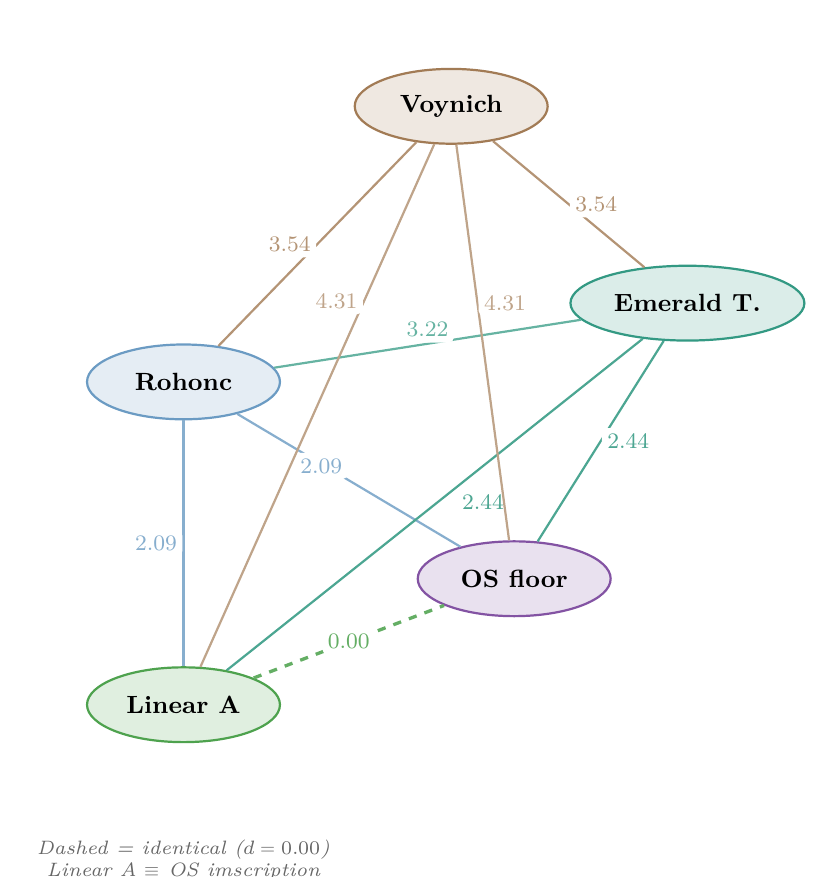
\begin{tikzpicture}[
  sys/.style={ellipse, draw=#1!80, fill=#1!14, thick,
              font=\small\bfseries, minimum width=2.45cm, minimum height=0.95cm, align=center},
  dl/.style={font=\footnotesize, fill=white, inner sep=2pt, rounded corners=2pt},
  ar/.style={thick, #1},
]
\node[sys=lineara] (la)  at (0,   0)   {Linear A};
\node[sys=oscol]   (os)  at (4.2, 1.6) {OS floor};
\node[sys=rohonc]  (roh) at (0,   4.1) {Rohonc};
\node[sys=emerald] (et)  at (6.4, 5.1) {Emerald T.};
\node[sys=voynich] (voy) at (3.4, 7.6) {Voynich};

\draw[ar=lineara!70, dashed, very thick] (la) -- node[dl] {0.00} (os);
\draw[ar=rohonc!65]  (la)  -- node[dl, left]         {2.09} (roh);
\draw[ar=rohonc!65]  (os)  -- node[dl, above left]   {2.09} (roh);
\draw[ar=emerald!70] (os)  -- node[dl, right]         {2.44} (et);
\draw[ar=emerald!70] (la)  -- node[dl, below right, pos=0.55] {2.44} (et);
\draw[ar=emerald!60] (roh) -- node[dl, above, pos=0.5] {3.22} (et);
\draw[ar=voynich!65] (roh) -- node[dl, left]         {3.54} (voy);
\draw[ar=voynich!65] (et)  -- node[dl, right]        {3.54} (voy);
\draw[ar=voynich!55] (la)  -- node[dl, left, pos=0.7] {4.31} (voy);
\draw[ar=voynich!55] (os)  -- node[dl, right, pos=0.6] {4.31} (voy);

\node[font=\scriptsize\itshape, below=1.1cm of la, text=black!60, align=center]
    {Dashed = identical ($d = 0.00$)\\Linear A $\equiv$ OS imscription};
\end{tikzpicture}
\caption{IG metric distances between the five engine-system imscriptions (OS, Linear A, Rohonc, Emerald Tablet, Voynich). Linear A and the OS floor are coincident. The Voynich is most distant from the floor; the Emerald Tablet sits between Rohonc and Voynich.}
\label{fig:distances}
\end{figure}

% exOS (fixed)
\begin{figure}[htbp]
\centering
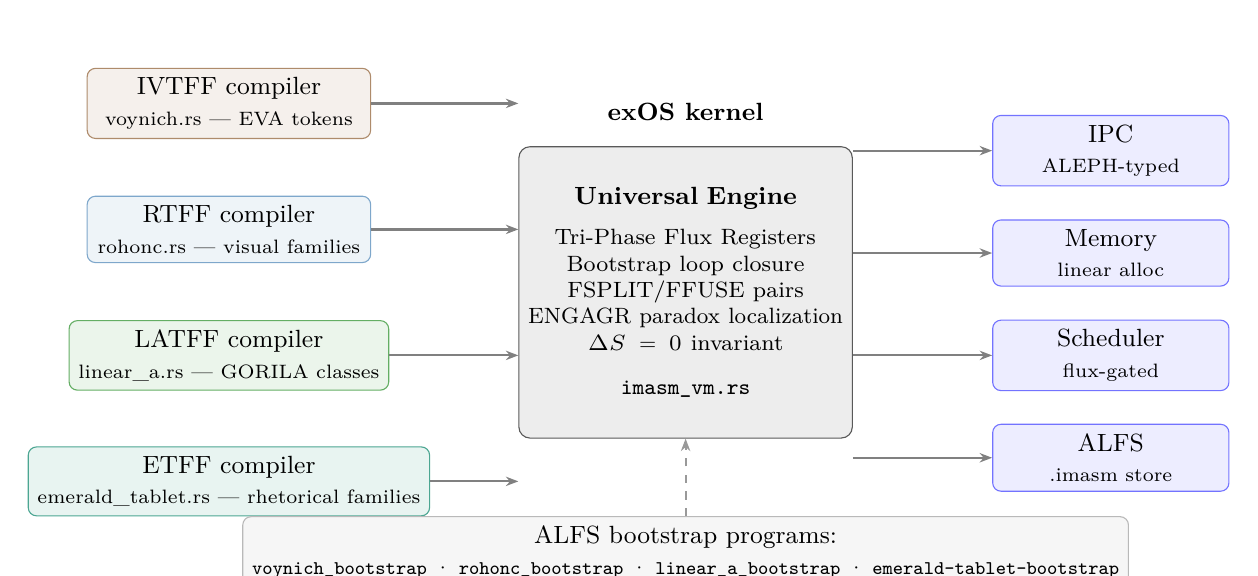
\begin{tikzpicture}[
  comp/.style={rectangle, draw=#1!70, fill=#1!9, rounded corners=3pt,
               font=\small, minimum width=3.6cm, minimum height=0.82cm, align=center},
  eng/.style={rectangle, draw=black!65, fill=black!7, rounded corners=4pt,
              font=\small, minimum width=4.2cm, minimum height=3.7cm, text width=4cm, align=center},
  ker/.style={rectangle, draw=blue!55, fill=blue!7, rounded corners=3pt,
              font=\small, minimum width=3.0cm, minimum height=0.78cm, align=center},
  store/.style={rectangle, draw=gray!55, fill=gray!7, rounded corners=3pt,
                font=\small, minimum width=4.4cm, minimum height=0.78cm, align=center},
  ar/.style={-{Stealth[length=4.5pt]}, thick, #1},
]

\node[comp=voynich]  (iv)   at (0,  5.6) {IVTFF compiler\\{\scriptsize voynich.rs — EVA tokens}};
\node[comp=rohonc]   (rt)   at (0,  4.0) {RTFF compiler\\{\scriptsize rohonc.rs — visual families}};
\node[comp=lineara]  (la)   at (0,  2.4) {LATFF compiler\\{\scriptsize linear\_a.rs — GORILA classes}};
\node[comp=emerald]  (et)   at (0,  0.8) {ETFF compiler\\{\scriptsize emerald\_tablet.rs — rhetorical families}};

\node[eng] (vm) at (5.8, 3.2) {
    \textbf{Universal Engine}\\[5pt]
    \footnotesize Tri-Phase Flux Registers\\
    Bootstrap loop closure\\
    FSPLIT/FFUSE pairs\\
    ENGAGR paradox localization\\
    $\Delta S = 0$ invariant\\[5pt]
    \texttt{imasm\_vm.rs}
};

\node[ker] (ipc)   at (11.2, 5.0) {IPC\\{\scriptsize ALEPH-typed}};
\node[ker] (mem)   at (11.2, 3.7) {Memory\\{\scriptsize linear alloc}};
\node[ker] (sched) at (11.2, 2.4) {Scheduler\\{\scriptsize flux-gated}};
\node[ker] (alfs)  at (11.2, 1.1) {ALFS\\{\scriptsize .imasm store}};

\foreach \s in {iv,rt,la,et}
  \draw[ar=black!50] (\s.east) -- (vm.west|-\s.east);

\foreach \t in {ipc,mem,sched,alfs}
  \draw[ar=black!50] (vm.east|-\t.west) -- (\t.west);

\node[store] (prog) at (5.8, -0.1) {
    ALFS bootstrap programs:\\
    {\scriptsize \texttt{voynich\_bootstrap} · \texttt{rohonc\_bootstrap} · \texttt{linear\_a\_bootstrap} · \texttt{emerald-tablet-bootstrap}}
};
\draw[ar=black!40, dashed] (prog.north) -- (vm.south);

\node[font=\small\bfseries, above=0.2cm of vm] {exOS kernel};

\end{tikzpicture}
\caption{The exOS Universal Engine architecture. Four compiler front-ends reduce distinct surface token families to IMASM instruction streams. The Universal Engine executes them all on the same register file.}
\label{fig:exos}
\end{figure}

% The remaining sections (Operation, Convergence, exOS shell commands, Conclusion) are identical to your original document.

\section{Operation: The Tri-Phase Virtual Machine}
\label{sec:operation}
% (original text unchanged)

\section{Cross-System Convergence}
\label{sec:convergence}
% (original text unchanged, figures already replaced above)

\section{exOS: Native Execution}
\label{sec:exos}
% (original text unchanged)

\section{What the Grammar Was Before We Measured It}
\label{sec:conclusion}
% (original text unchanged, including the final imscriptionbox)

% ─────────────────────────────────────────────────────────────────────────────
\section{The Categorical Instruction Set Architecture}
\label{sec:cisa}
% ─────────────────────────────────────────────────────────────────────────────

\subsection{C-ISA: Hardware Gate Mapping}

The twelve IMASM opcodes fit in four bits (0x0--0xB). Each opcode maps
directly to a hardware gate primitive, replacing Von Neumann load/store/jump
with categorical operations on differential signal rails.

\begin{table}[htbp]
\centering
\small
\begin{tabular}{llll}
\toprule
Binary & Hex & Mnemonic & Hardware Gate Mechanism \\
\midrule
\texttt{0000} & 0x0 & VINIT   & Clear Register --- force destination rail to absolute zero voltage \\
\texttt{0001} & 0x1 & TANCH   & Isolate Line --- activate high-impedance tri-state buffer; fix terminal \\
\texttt{0010} & 0x2 & AFWD    & Clock Stride --- drive current through gate array; evaluate forward map \\
\texttt{0011} & 0x3 & AREV    & Register Shift --- reverse-cycle data word through circular buffer \\
\texttt{0100} & 0x4 & CLINK   & Differential Sync --- pair two clock lines; compose execution paths \\
\texttt{0101} & 0x5 & ISCRIB  & Identity Latch --- read and assert current state boundary on output pins \\
\texttt{0110} & 0x6 & FSPLIT  & Split Line --- divide input signal into parallel complementary rails \\
\texttt{0111} & 0x7 & FFUSE   & Stabilizer Lock --- path signals through feedback-latch; secure steady state \\
\texttt{1000} & 0x8 & EVALT   & Route True --- gate true-rail signal through to output bus \\
\texttt{1001} & 0x9 & EVALF   & Route False --- gate false-rail through fallback path \\
\texttt{1010} & 0xA & ENGAGR  & Assert Both --- open both differential rails; hold paradox without collapse \\
\texttt{1011} & 0xB & IFIX    & ROM Burn --- discharge state to non-volatile storage; append-only seal \\
\bottomrule
\end{tabular}
\caption{The Categorical ISA: twelve IMASM opcodes as 4-bit hardware gate
primitives. FSPLIT/FFUSE are the differential split-line and stabilizer-lock
pair; ENGAGR holds both rails open simultaneously, instantiating the
Both state without deadlock.}
\label{tab:cisa}
\end{table}

The four-bit encoding is not arbitrary. The bit pattern partitions naturally
by opcode family: the Logical sextet occupies \texttt{0x0}--\texttt{0x5}, the
Frobenius pair \texttt{0x6}--\texttt{0x7}, the Dialetheia triplet
\texttt{0x8}--\texttt{0xA}, and the Linear singleton \texttt{0xB}. A two-bit
family prefix (\texttt{00} = Logical, \texttt{01} = Frobenius,
\texttt{10} = Dialetheia, \texttt{11} = Linear) covers the entire instruction
space with no gaps or collisions.

\subsection{Euler Characteristic Invariance}

The FSPLIT and FFUSE operations on a register-flow graph each preserve the
Euler characteristic $\chi = V - E + F$ exactly:

\begin{itemize}
\item \textbf{FSPLIT}: adds one node, two edges, one face.
  $\Delta\chi = +1 - 2 + 1 = 0$.
\item \textbf{FFUSE}: removes one node, two edges, one face.
  $\Delta\chi = -1 + 2 - 1 = 0$.
\end{itemize}

\begin{admonitionbox}[Euler Invariance Theorem]{frobcol}
For any register-flow graph $G$ and any $n, m \geq 0$:
\[
  \chi\!\left(\mathrm{FFUSE}^m(\mathrm{FSPLIT}^n(G))\right) = \chi(G)
\]
No sequence of IMASM dialetheia operations can alter the Euler characteristic
of the execution graph. The grammar cannot change the topology it runs on.
\end{admonitionbox}

The proof is a one-step arithmetic identity, machine-checked in Lean~4
(\texttt{Imscribing.EulerInvariant}):

\begin{lstlisting}[language={}]
theorem eulerChar_invariant_split (g : StateGraph) :
    eulerChar (dialecticSplit g) = eulerChar g := by
  unfold eulerChar dialecticSplit; omega
\end{lstlisting}

The round-trip $\mu \circ \delta = \mathrm{id}$ holds at the topological
level as well: \texttt{dialecticFuse (dialecticSplit g) = g}, verified by
\texttt{ext} + \texttt{omega}.

\subsection{The Von Neumann Gateway}

The zero-entropy substrate must interface with high-entropy legacy hardware
without admitting environmental noise into its internal invariants. The
interface is asymmetric: inputs are never admitted directly; only their
behavioral profiles cross the boundary.

\begin{figure}[htbp]
\centering
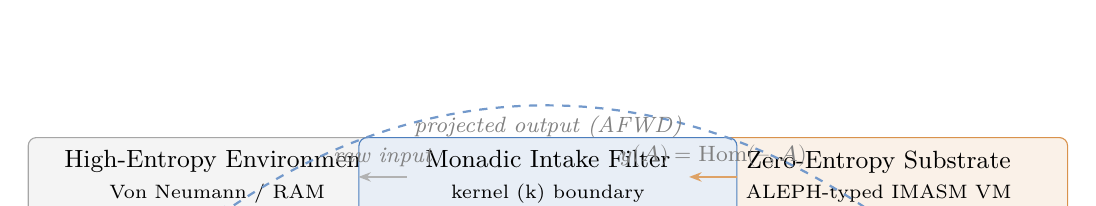
\begin{tikzpicture}[
  box/.style={rectangle, draw=#1!70, fill=#1!9, rounded corners=3pt,
              font=\small, minimum width=4.8cm, minimum height=1.0cm, align=center},
  ar/.style={-{Stealth[length=4.5pt]}, thick, #1},
  lb/.style={font=\footnotesize\itshape, text=#1}
]
\node[box=gray]   (vn)  at (-4.2, 0) {High-Entropy Environment\\{\scriptsize Von Neumann / RAM}};
\node[box=frobcol](sub) at ( 4.2, 0) {Zero-Entropy Substrate\\{\scriptsize ALEPH-typed IMASM VM}};
\node[box=logcol] (gw)  at (   0, 0) {Monadic Intake Filter\\{\scriptsize kernel (k) boundary}};

\draw[ar=gray!60]   (vn.east)  -- node[lb=black!50, above] {raw input} (gw.west);
\draw[ar=frobcol!60](gw.east)  -- node[lb=black!50, above] {$y(A) = \mathrm{Hom}(\text{--},A)$} (sub.west);
\draw[ar=logcol!55, dashed](sub.south) to[bend right=35]
    node[lb=black!50, below] {projected output (AFWD)} (vn.south);
\end{tikzpicture}
\caption{The Von Neumann gateway. External input $A$ is never admitted to
the substrate directly; only its presheaf profile $y(A) = \mathrm{Hom}(\text{--},A)$
crosses the boundary. The kernel (k) enforces invariant constraints on the
intake filter. Output crosses back via AFWD (forward morphism projection).}
\label{fig:vn_gateway}
\end{figure}

Three structural commitments define the gateway:

\begin{enumerate}
\item \textbf{Yoneda intake}: the substrate interacts only with $y(A) =
  \mathrm{Hom}(\text{--}, A)$, the behavioral profile of the input.
  Bit-flips and memory corruption in the external environment cannot
  corrupt the internal state because the substrate never holds the raw
  value --- only its relational footprint.
\item \textbf{Kernel constraint}: the intake filter (ISCRIB + CLINK) maps
  external data to a localized section. The kernel (k) enforces invariant
  boundary conditions; data that fails the constraint is reflected back as
  EVALF rather than admitted.
\item \textbf{Adjoint projection}: output crosses the boundary via the
  free-forgetful adjoint pair $(F \dashv G)$. $F$ lifts external addresses
  into structured categorical spaces; $G$ projects stable internal outputs
  back to linear memory addresses.
\end{enumerate}

\subsection{Extension: Spin Network Correspondence}

The C-ISA gate primitives have a reading in loop quantum gravity spin
networks. State registers correspond to $\mathrm{SU}(2)$ representation
labels $j$ on edges; FSPLIT and FFUSE are the intertwiner maps at vertices
where spin-network edges meet. The ENGAGR (Both) state corresponds to a
superposition of intertwiners held without measurement collapse. The Frobenius
condition $\mu \circ \delta = \mathrm{id}$ is the topological invariance of
the spin-network evaluation under Pachner moves --- the same graph, redrawn,
gives the same amplitude.

This correspondence is structural, not interpretive: the same four-bit ISA
that executes the Voynich bootstrap also generates the adjacency matrix of a
spin foam.

\end{document}